\documentclass[12pt,a5paper,twoside]{article}

\usepackage{times}
\usepackage{verse}
\usepackage{cmap}
\usepackage{pscyr}
\usepackage{float}
\usepackage{epigraph}
\usepackage[T2A]{fontenc}
\usepackage[utf8]{inputenc}
\usepackage{graphicx}
\usepackage[english,russian]{babel}
\usepackage{textcomp}
%для сложной нумерации страниц
\usepackage[strict]{changepage}
\usepackage{setspace}
%так мы меняем шрифт. 
\renewcommand{\rmdefault}{fac}
\renewcommand{\poemtoc}{subsection}
\newcommand{\blankpage}{
\newpage
\thispagestyle{empty}
\mbox{}
\newpage
}
\setlength{\epigraphrule}{0pt}
\setlength{\epigraphwidth}{.5\columnwidth}
%\makeatletter
%\renewcommand{\@evenhead}{}
%\renewcommand{\@evenfoot}{}
%\makeatother

%\oddsidemargin=-10mm
%\textwidth=123mm
%\topmargin=-25mm
%\textheight=170mm

%геометрию страницы так гораздо удобнее менять
\usepackage{geometry}
\geometry{left=1.5cm}
\geometry{right=1.5cm}
\geometry{top=2cm}
\geometry{bottom=2cm}


\newcommand{\attrib}[1]{\nopagebreak{\raggedleft\footnotesize #1\par}}
\newcommand{\pict}[1]{\thispagestyle{empty}\begin{figure}[H]\begin{center}\includegraphics[width=1\linewidth]{#1}\end{center}\end{figure}\newpage}
\hyphenation{по-вест-во-ва-те-ля}
\begin{document}

\setcounter{page}{5}

%% >>>>>>>>>>>>>>>> Что сделать <<<<<<<<<<<<<<<<<<<
%%%%>>>>>>>>>>>>>>>>>>>>>>>>>С этими картинками делаем так: я вначале верстаю текст, потом отдельно вставляю обложку и этот пироскаф. там же не нужны ни нумерация, ни поля. 
%pdftk oblogka-1.pdf title.pdf title2.pdf pyroskaf-1.pdf [основной текст] oblogka-2.pdf pyroskaf-2.pdf output final_book.pdf
% надо заверстать основной текст (где стихи) в блок и сказать не нумеровать четные (или нечетные, не помню) страницы. вступление и заключение оставить как есть. 
% выровнять все картинки 
% сделать титул и оглавление (которе непонятно как делать, ведь наш текст не разбит на разделы итп...)




%\begin{figure}[H]
%\begin{center}
%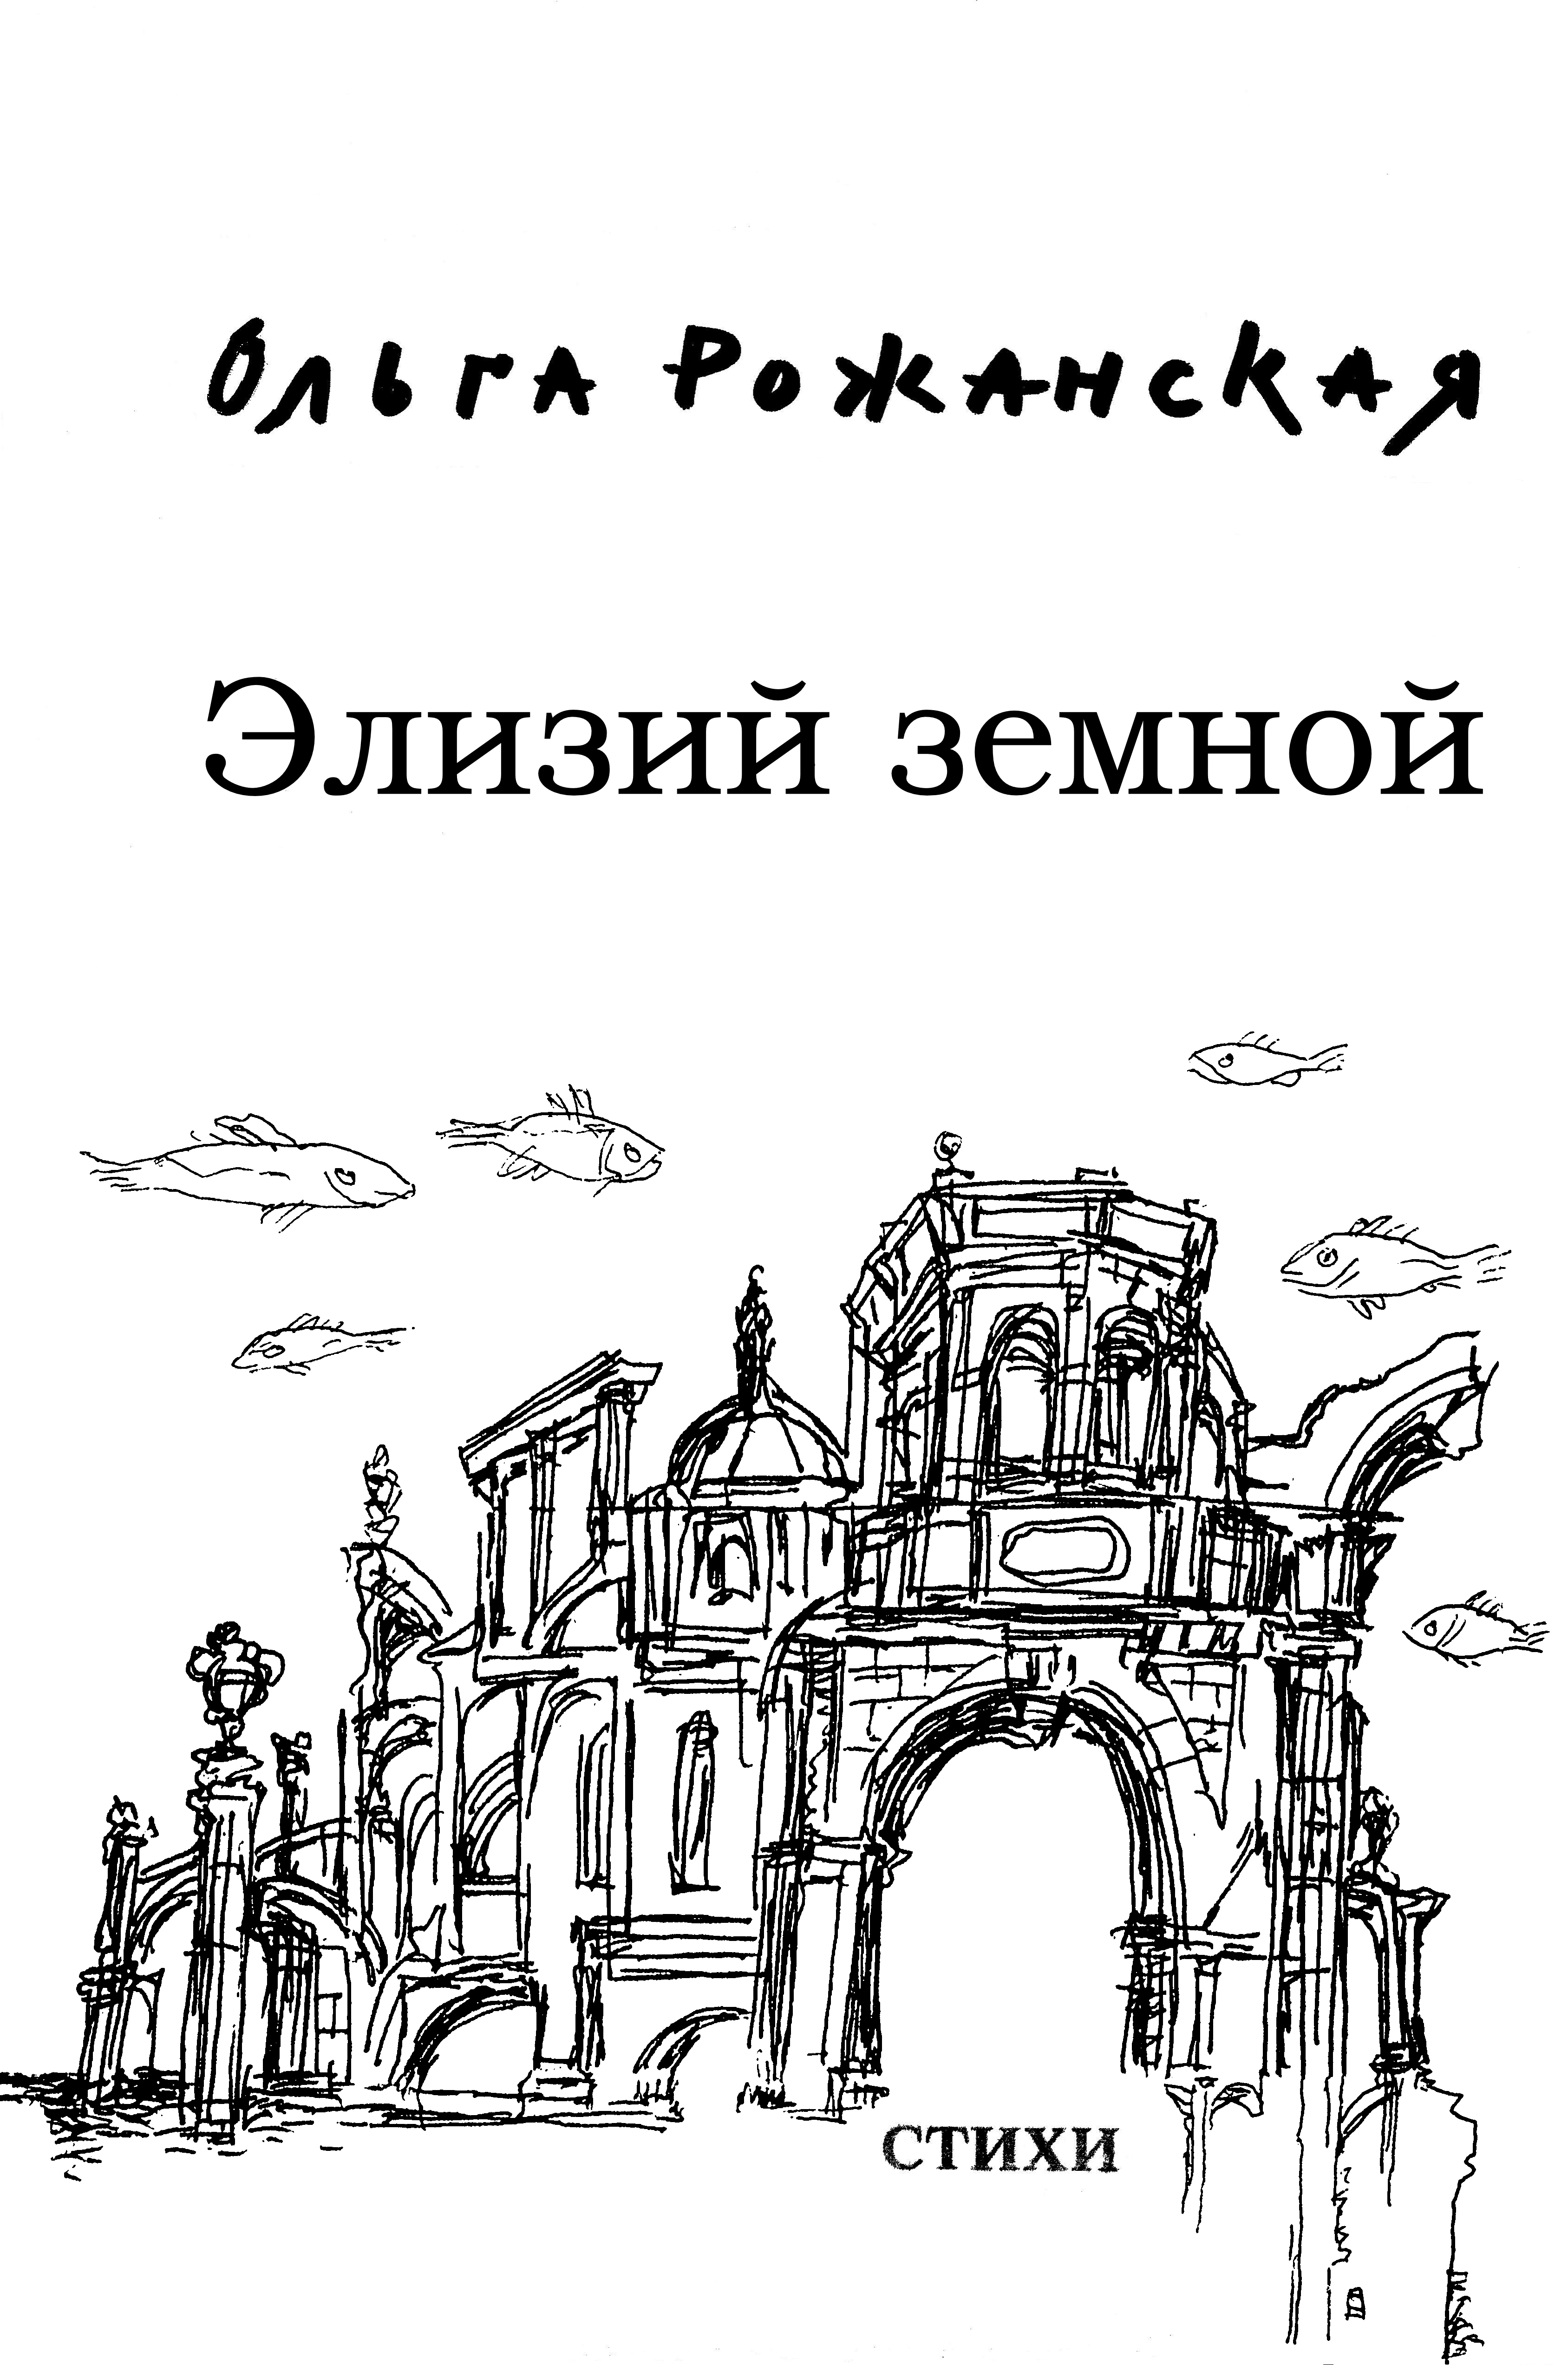
\includegraphics[width=1\linewidth]{picts/oblogka1.png} 
%
%\end{center}
%\end{figure}
%\enlargethispage{3\baselineskip}


%\begin{figure}[H]
%\begin{center}
%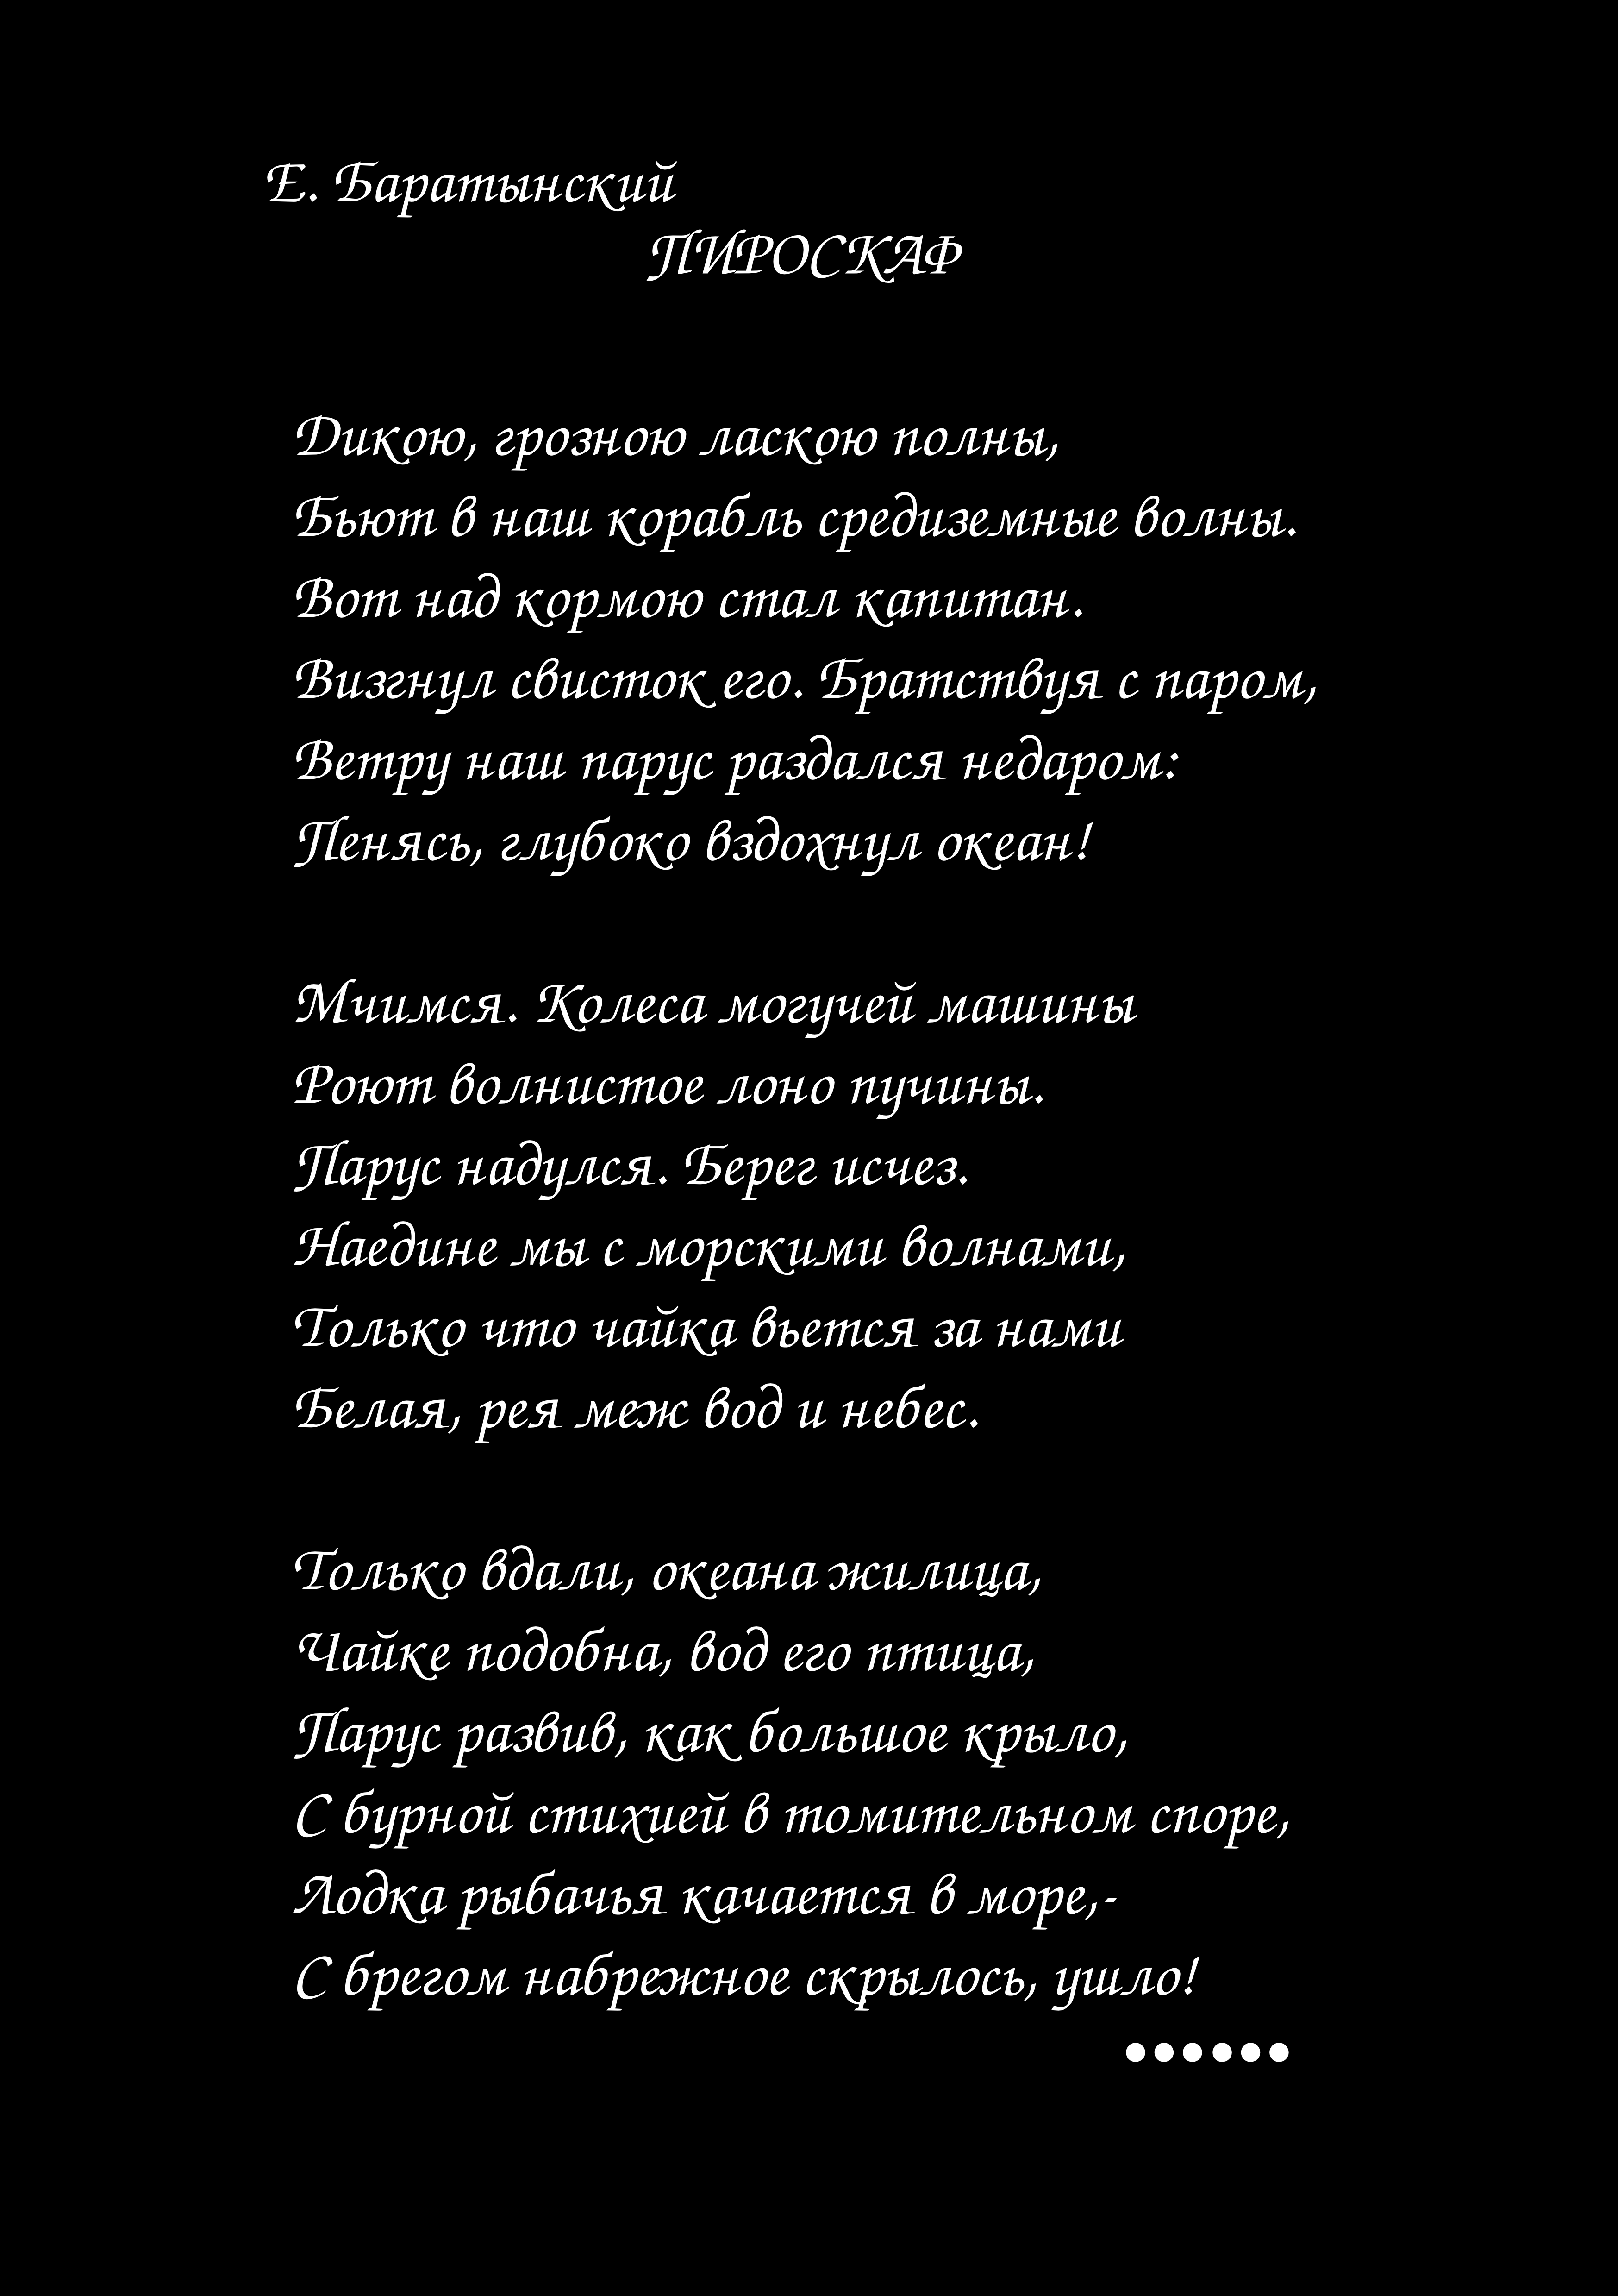
\includegraphics[width=1\linewidth]{picts/pyroskaf-1.png} 
%\end{center}
%\end{figure}






%----------------------------------------------------------------------
\begin{center}
\subsubsection*{Голос}
\addcontentsline{toc}{section}{\textit{Кирилл Анкудинов}. Голос}
\end{center}

Писать об этой книге трудно.

Не так-то легко даже читать её.

В этой книге -- как во всех поэтических сборниках Ольги Рожанской -- музеум всех времён и народов.

Колыбель Христианства -- ветхозаветная Иудея (Ольга Рожанская часто писала о мире Ветхого Завета; 
Новый Завет для неё почти неназываем, апофатичен). Христианская ойкумена -- средневековая Франция, 
старая Англия, Московская Русь. Дохристианские цивилизации 
(греческая Античность, Скандинавия конунгов), внехристианские цивилизации 
(Шумер, Древний Египет, Китай).

В этой книге Ольги Рожанской стихи -- ещё сложнее для читательского восприятия, чем стихи её предыдущих книг.

В произведениях на историческую тематику всегда должна быть экспозиция, 
вводящая читателя (слушателя, зрителя) в место и время действия. Театральная декорация. 
Портик с ионическими колоннами на переднем плане, панорама Афин на заднем плане -- стало быть, 
мы в Древней Греции. Повсюду египетские иероглифы -- значит, мы в Древнем Египте. 
В литературе роль ``декораций'' играют исторические реалии, имена, детали, специально 
введённые автором в начальные абзацы произведения.

В стихотворениях этой книги такие реалии могут появиться в самой последней строфе. 
Или не появиться вообще.
Мы, читатели, не пребываем в уютно освещённом зрительном зале, 
мы пробираемся среди декораций в ночной темноте -- с фонариком. Хорошо ещё, 
если луч нашего фонарика выхватит из мрака амфору или резную балясину. 
А то ведь придётся на ощупь догадываться о том, где мы сейчас 
находимся -- в Древней Греции, в Вавилоне или в современной Москве.

\newpage
% ****************
\settowidth{\versewidth}{Над водой слышнее звуки,}
\begin{verse}[\versewidth]
Над водой слышнее звуки, \\
Небо тонет в тростниках.\\
К небу кто протянет руки --\\
Тоже канет в тростниках.

Над водой бесцветной рябью\\
Всеми ста проходит Дух.\\
Тверди где восстать над хлябью --\\
Все места обходит Дух.

Высшей Силы деликатность\\
Воды сдержит, если мы\\
На ногах своих, на ватных,\\
Робко выступим из тьмы.
\end{verse}
% ****************

Из двух первых строф этого стихотворения не ясно почти ничего. Тростники. Египет? 
А, может и не Египет (мало ли где растут тростники). Дух, отделяющий твердь от водной хляби. 
Ветхий Завет? Не обязательно (в полинезийских мифах Бог тоже отделяет сушу от вод). 
Только третья строфа более-менее определённо наводит на исходный сюжет. Кажется, 
здесь речь идёт о египетском пленении евреев и об их исходе через Чермное (Красное) море. 
Но именно что кажется -- с большой, но не с окончательной уверенностью.

А порой вообще нет даже малейших подсказок…

% ****************
\settowidth{\versewidth}{Посмотри на восток:}
\begin{verse}[\versewidth]
Посмотри на восток:\\
Так ли ветер, как прежде, жесток?\\
И на запад взгляни:\\
Потонули иль живы они?
\newpage
Шелестя, как песок,\\
Уползает за часом часок.\\
Словно дети в лесу,\\
Мы ужасную зрели красу --

Плыли змеи в ночи\\
И луны отражали лучи.
\end{verse}
% ****************

Кто --- ``они'' (потонувшие или не потонувшие)? Что за змеи плыли в ночи?

Чтобы понять, о чём ведётся разговор, придётся заглянуть в словарь ``Мифы народов мира''. 
Да и тот не поможет (слишком многие народы мира свидетельствовали о змеях, плывущих в ночи).

Какой-то слепой обломок неведомой мифологии, археологический артефакт без перспективы 
на верную атрибуцию.
 Стихи этой книги -- словно уравнения с большим количеством 
неизвестных, иксов и игреков. Иногда, кстати, и иксов-то не столь много, но всё равно решение не просматривается.

% ****************
\settowidth{\versewidth}{Вот Папа, в том не ведая греха,}
\begin{verse}[\versewidth]
Вот Папа, в том не ведая греха,\\
Пощупал пленников, лежащих на рогоже:\\
``Ну, точно ангелы! -- полны и светлокожи.\\
Чтоб выбить дурь, пошлём к ним пастуха''.

У них на севере шумит широкий дуб.\\
Ты варварской душе придай ветвисту форму;\\
Простую пищу ешь (у нас так скот не кормят!),\\
И капища не тронь наивный сруб.
\end{verse}
% ****************

Попытка обратить в католическую веру северных язычников 
(Папа шлёт к ним посланника и даёт ему назидания)? Допустим. 
Но о каких именно язычниках идёт речь -- о германцах, кельтах, балтах, славянах? Неясно.

Да тут ещё и характерно сверхплотный синтаксис поэзии Ольги Рожанской, вполне достойный царственного синтаксиса Вячеслава Иванова.

``Его суровые речения сцеплены крепко, - местами они кажутся даже скованными… И мне до горечи обидно… за недоступность так заманчиво пляшущих передо мной хореев и за 
тайнопись их следов на арене, впитавших столько благородного пота''.

(Иннокентий Анненский. <<О современном лиризме>>).

Редкие конкретные существительные --- тростники, дубы и туманы --- впаяны в железные 
конструкции неведомого нам контекста и укрупнены до предела. 
Маленький человек неуклюже тыкается во все эти тростники, дубы и туманы.

Наталкиваясь на Бога.

Поэзия Ольги Рожанской -- религиозная, духовная поэзия.

Но она не похожа на обычную религиозную поэзию -- как классическую, так и современную. 
Непохожа на поэзию Олеси Николаевой, Светланы Кековой, даже на поэзию Ольги Седаковой 
(я уж не говорю о песнопениях Жанны Бичевской или иеромонаха Романа).

Если обычная религиозная поэзия -- уверенно-линейный диалог автора с Богом, 
то пунктирные стихи Рожанской -- нечто совсем иное. Я бы сказал, что это напоминает
мне попытки землян установить контакт с внеземными цивилизациями.

Земляне шлют в космос сигналы -- без какого то ни было подтверждения, 
что эти сигналы приняты (и могут быть приняты в принципе). Земляне, 
в свою очередь, то ли получают, то ли не получают некие ``свидетельства'' 
от инопланетян, но невозможно достоверно выяснить, чего стоят 
данные свидетельства, и, тем более, что конкретно они означают.

Оттого так смутны стихи Ольги Рожанской, ведущиеся от лица многих
людей или от лица одного человека (даже если этот человек -- Пророк, исполняющий волю Господа).

Горизонт читателя в этих стихах соответствует горизонту по\-вест\-во\-ва\-те\-ля-простеца -- вот 
именно слепо тыкающегося в тростники, дубы и туманы, в эллинские побережья и 
норвежские фьорды, в британские холмы и московские высотки.

Есть в этой книге Ольги Рожанской и иные стихи -- написанные
от Имени Бога (чаще всего, хоть не всегда -- от имени Бога Ветхого Завета).

Воистину, державинское дерзновение.

% ****************
\settowidth{\versewidth}{Я отманил Лавана дочерей,}
\begin{verse}[\versewidth]
Я отманил Лавана дочерей,\\
Как голубиц с соседней голубятни.\\
Изобрази, чтоб было им понятней,\\
Вола и льва у храмовых дверей.

Веди, пророк, непонятую речь;\\
Паси слова, как Я пасу народы.\\
Пока с глагола справишься породой,\\
Успею кости кожею облечь.

Побив раба и нагрузив осла,\\
Ты хочешь знать зачем земля кругла?\\
Поди спроси богов своих голодных!\\
Я ночь черню. Чудны Мои дела.
\end{verse}
% ****************

Бог сам признаётся в том, что чудны Его дела 
(и вправду -- инопланетянин). Да ещё и с ревнивой насмешкой отсылает пророка 
к его богам (<<Поди спроси богов своих голодных>>).

Это ещё что: в некоторых стихах Ольги Рожанской (Единый) Бог сам способен творить (множественных) богов.

% ****************
\settowidth{\versewidth}{Иная близится пора,}
\begin{verse}[\versewidth]
Иная близится пора,\\
И руки взъемлют рукояти;\\
От нас неведенье отъяти\\
Задумал Ты. И рек: ``Пора!''
\newpage
И вот -- наполнен небосвод,\\
Как хлев, сварливыми богами,\\
И властелин вперёд ногами\\
В ладье украшенной плывёт.
\end{verse}
% **************** 

Поэзия Ольги Рожанской -- христианская поэзия. Но она, эта поэзия, 
абсолютно лишена ``конфессиональной самозамкнутости'' и неизбежного следствия такой замкнутости -- ``конфессионального эгоизма''.

Тут не то что ``перегородки между верованиями не доходят до Бога''; 
тут Бог Сам творит эти перегородки по Свой Воле (и Сам их разрушает по Своей Воле).

Бог, например, может сделать человеку языческую веру -- исходя из состояния духа и сознания человека, 
подобно тому, как отец делает своему ребёнку яркую игрушку.

И даже ``эволюция по Дарвину'' - не более чем ещё одна игрушка Бога для любимого дитяти (для человека).

% ****************
\settowidth{\versewidth}{Грядет Великая Игра.}
\begin{verse}[\versewidth]
Грядет Великая Игра.\\
Земная корчится кора,\\
И проявляются черты\\
Лица Того, с кем мы -- на ``ты''.

Смотри: по правилам игры\\
Скачками движутся миры,\\
И превращается в змею\\
Амёба, суть слиняв свою.

Выходят крабы из пучин,\\
Чтоб веселиться без причин,\\
И перед сушей пляшет кит,\\
Как перед скинией Давид.
\end{verse}
 % ****************
 
В духовной лирике Ольги Рожанской светлый луч Благой Вести -- как бы проходит сквозь стёкла, 
призмы и витражи человеческого сознания, преломляясь и расщепляясь на сотни многоцветных лучиков.

Я впервые употребил слово ``лирика'' - и тут же усомнился в правомочности этого.

Как известно, не всякая поэзия -- лирика (да и не всякая лирика -- поэзия).

Лирика -- всё, что написано от себя, от собственной души. Пускай даже от имени приукрашенного ``лирического героя'' - но всё равно от себя.

Потому поэма Александра Твардовского ``Страна Муравия'' - не лирика. 
И роман ``Евгений Онегин'' - лирика лишь в лирических отступлениях.

Ольга Рожанская, в основном, писала не от себя; её стихи -- либо речь из 
уст ``другого'' (египетского жреца, древнего грека, средневековой дамы, пророка, Бога), 
либо безличное повествование. В этой книге я насчитал только четыре стихотворения, 
написанных автором от себя (плюс ещё четыре стихотворения -- под сомнением).

Лирика ли -- этот великолепный монотеатр Ольги Рожанской, в котором одна-единственная исполнительница, но так много разнообразных ролей?

Да, лирика.
Во-первых, лирическое начало обеспечено личностью 
автора -- удивительно цельной и зримо проглядывающей
сквозь все пёстрые маски и стилизации.

А во-вторых…

Этот сборник стихов -- посмертная книга Ольги Рожанской. Нельзя не учитывать это.

Дело даже не в том, что ``когда человек умирает, меняются его портреты''.

Дело в другом…

Мне очень неудобно говорить то, что я скажу сейчас…

Боюсь впасть в грех ``крайнего эстетизма, доходящего до бесчеловечности''.

Тем не менее, скажу…

Мне кажется, что трагическая смерть Ольги Рожанской стала завершением композиции этой книги.

Словно купол на храме.

Понимаю, что это моё заявление -- более чем рискованно. Поддержкой полагаю слова, услышанные 
мной от виднейшего православного богослова наших дней -- протодиакона о. Андрея (Кураева): 
``Каждый человек должен работать над будущей собственной смертью, словно над произведением искусства''.

(Разве не явления культуры и искусства -- смерти Державина, Пушкина, Лермонтова, 
Льва Толстого, Чехова, Блока, Александра Меня?).

…Эта тема в этой книге прозвучит два раза.

Первый раз -- тихо, спокойно, трезво, мудро…

% ****************
\settowidth{\versewidth}{Я не скажу, чтоб я жила счастливо,}
\begin{verse}[\versewidth]
Я не скажу, чтоб я жила счастливо,\\
А всё ж не так, чтоб не хотеть еще!\\
Кто дал нам право требовать добавки?\\
(Метели мягкой и колючей травки)\\
О если б жизнь подвергнуть строгой правке,\\
Ведя слогам связующий подсчёт!

Открой глаза, гляделки, очи, вежды:\\
Ты видишь мир, снимающий одежды.\\
Спектакль сыгран. Брось свои надежды\\
На третий бис, настырный человек!
\end{verse}
% ****************

Обычное пророчество поэта. Из того же ряда, что и ``с свинцом в груди лежал недвижим я…'' или ``я умру в крещенские морозы…'' (вот ещё: майкопская поэтесса Татьяна Оленина начала своё стихотворение: ``Я умру весною ранней'' - и умерла в марте).

Быть пророком -- это так естественно, так легко для поэта. Обыкновенное чудо (чудо -- но обыкновенное; всего лишь чудо).

Но вот -- совсем иное…

% ****************
\settowidth{\versewidth}{Возьми, Господь, поля и реки,}
\begin{verse}[\versewidth]
Возьми, Господь, поля и реки,\\
Как пищу, поднеси к устам.\\
(И дол ревёт, и тают снеги,\\
И дрожь взбегает по листам).

Возьми, Господь, мечты и цели;\\
Меж “Ты” и  “Я” заполни брешь,\\
И, как Твое мы Тело съели,\\
Ты наши устремленья съешь.

Уйми страстей своих бурленье,\\
Душа! Я посмотреть хочу,\\
Как выпрямляются растенья\\
Навстречу первому лучу.
\end{verse}
% ****************
  
Этот потрясающий, испепеляющий, бьющий наотмашь пасхальный псалом-крик -- самое последнее стихотворение Ольги Рожанской, написанное ею за неделю до гибели.

Не знаю, как мне это комментировать и возможно ли комментировать вообще.

Такого не было во всей русской литературе. Да и во всей мировой литературе, думаю, тоже.

Это -- не ``страница из истории литературы''; это момент бытия Духа…
%\begin{minipage}{\textwidth}
\begin{flushright}
Кирилл Анкудинов, 2011 г.
\end{flushright}
%\end{minipage}
\newpage
\pict{picts/zastavka.png} 
\begin{center}
\bigskip
\thispagestyle{empty}
\vspace*{3cm}
\Huge{Стихотворения}
\end{center}
\addcontentsline{toc}{section}{Стихотворения}

\newpage

%--------------------------------------------------------------------------------------------------------------------
%Сюда вставлять стихи в отм порядке, в котором они должны идти
\pict{picts/Gestokiy_romans1.png} 
\poemtitle{Жестокий романс}
\settowidth{\versewidth}{На груди, на седой, на курчавой,}
\begin{verse}[\versewidth]
На груди, на седой, на курчавой,\\
Дядя Гриша свой крестик несёт,\\
Словно лодку на привязи водит,\\
Словно в поле овечку пасёт.

Раньше людям он чистил ботинки\\
У Дворца, на проспекте Труда;\\
И от будки вели по старинке\\
Две доски – неизвестно куда.

В пузырьках из-под пенициллина\\
Разноцветных эмалей ряды\\
Наблюдали, как двадцать копеек\\
Вы давали ему за труды.

А теперь он живёт на покое,\\
И как примет четыреста грамм –\\
Во дворе с шестиклассником Колей\\
Обсуждает гуляющих дам.

Коля дома имеет компьютер,\\
Что ни кушать не просит, ни пить,\\
Но персидского принца не любит\\
Он по комнатам страшным водить.

Потому что в пузатых бутылках,\\
Осушаемых часто до дна,\\
Много жизней скопилось у принца,\\
А у них с дядей Гришей –\\
\begin{minipage}{0.45\textwidth}
\begin{flushright}
		– одна!
\end{flushright}
\end{minipage}
\end{verse}

\newpage
\pict{picts/Kto_raspryag1.png} 

		
\poemtitle[Кто распряг семизвездный Воз]{* * *}
\settowidth{\versewidth}{Кто распряг семизвездный Воз}
\begin{verse}[\versewidth]
Кто распряг семизвездный Воз\\
И пошёл поразмять ступни?\\
Если в мире не станет звёзд,\\
Завопит глубина земли.

Из глубин подземной горы\\
Вулканический спросит князь:\\
”Пока  спал, кто сожрал миры,\\
Что, как птицы, пели, смеясь?”

Покатился на запад Воз.\\
(То из гроба везут царя),\\
И Подпасок, Охотник, Пёс\\
Следом в гору бегут, горя.
\end{verse}
\newpage


\pict{picts/Ya_otmanil.png} 


\poemtitle[Я отманил Лавана дочерей]{* * *}
\settowidth{\versewidth}{Я отманил Лавана дочерей,}
\begin{verse}[\versewidth]		
Я отманил Лавана дочерей,\\
Как голубиц с соседней голубятни.\\
Изобрази, чтоб было им понятней,\\
Вола и льва у храмовых дверей.

Веди, пророк, непонятую речь;\\
Паси слова, как Я пасу народы.\\
Пока с глагола справишься породой,\\
Успею кости кожею облечь.

Побив раба и нагрузив осла,\\
Ты хочешь знать зачем земля кругла?\\
Поди спроси богов своих голодных!\\
Я ночь черню. Чудны Мои дела.
\end{verse}
\newpage

\pict{picts/Na_svadbu_piva1.png} 


\poemtitle[На свадьбу пива нового не сваришь]{* * *}
\settowidth{\versewidth}{На свадьбу пива нового не сваришь,}
\begin{verse}[\versewidth]		
На свадьбу пива нового не сваришь,\\
Пока созвездий не закончен ряд.\\
Я море жму, как жмых. “Держись, товарищ!” –\\
Края земли друг другу говорят.

Кузнец сказал: “Ты глину мял ногами,\\
А я расправил молотом листы”.\\
Меж жизненным и смертным берегами,\\
Как пьяный Ной, раскинулись мосты.

“Подобно ивам при потоках вод,\\
Жестковыйный посажу народ.\\
И жалость, отраженная в воде,\\
Расскажет им о Правде и Суде”.
\end{verse}
\newpage
\pict{picts/Ti_ne_plach1.png} 


\poemtitle[Ты не плачь, не плачь, Маруся]{* * *}
\settowidth{\versewidth}{Ты не плачь, не плачь, Маруся,}
\begin{verse}[\versewidth]
Ты не плачь, не плачь, Маруся,\\
По-над жизнию своей!\\
Над рекой летели гуси,\\
Воды сделались белей.

Следом утки полетели,\\
Следом – стая лебедей.\\
Своды райские вспотели\\
От дыхания людей.

Тут перила завитые,\\
Разноцветное стекло,\\
Носят строгие святые\\
В сердце грозное тепло.

Не рыдай же ты, Маруся;\\
(Развела здесь бабий вой.)\\
Дай я Богу помолюся\\
Перед дверью гробовой.
\end{verse}
\newpage
\pict{picts/Eto_moya_zemla1.png} 


\poemtitle[Это моя земля]{* * *}
\settowidth{\versewidth}{Это моя земля.}
\begin{verse}[\versewidth]
Это моя земля.\\
Воздух еще не сжат.\\
Вздыбленные поля\\
неба – белы лежат.

Впившиеся любви\\
путы – ослабь слегка!\\
Видишь? – За мной пришли\\
Белые облака.
\end{verse}
\newpage

\pict{picts/stixi_pokoynogo_poeta1.png} 


\poemtitle[Стихи покойного поэта]{* * *}
\settowidth{\versewidth}{Стихи покойного поэта}
\begin{verse}[\versewidth]
Стихи покойного поэта\\
Читаю в книжице посмертной.\\
Он был веселым человеком\\
И жил неподалеку где-то.

Как поднимаются туманы\\
От поля млечного, парного!\\
И отражается сосновый\\
Лесок – в прозрачном небосводе.

А про покойного поэта\\
Скажу не мало и не много:\\
Он жил неподалеку где-то\\
И, кажется, поверил в Бога.
\end{verse}

\newpage

\pict{picts/Na_mira_xram.png} 


\poemtitle[На мира храм ложится первый снег]{* * *}
\settowidth{\versewidth}{На мира храм ложится первый снег.}
\begin{verse}[\versewidth]
На мира храм ложится первый снег.\\
Потише там! – чихнул, и кончен век.\\
(Дрожит дуга, несущая светила.)\\
Мы – рыбы; нас морозцем прихватило;\\
Бежит слеза из глаз, лишенных век.

Проходит свет рассеянный сквозь лёд.\\
Звездами свод усеянный – поёт.\\
Мерцает мерно Океана глыба.\\
В глубинных стойлах, стоя, дышат рыбы.\\
Пройдёт столетье – рыбина моргнёт.
\end{verse}
\newpage

\pict{picts/Iz_tmy_gospod.png} 


\poemtitle[Из тьмы Господь призвал меня]{* * *}
\settowidth{\versewidth}{Из тьмы Господь призвал меня.}
\begin{verse}[\versewidth]
Из тьмы Господь призвал меня.\\
(Не мни: его безумны речи!)\\
Я Славу видел средь огня\\
И Слово съел, как сыр овечий.

Молчи, пока Я говорю!\\
Я прилепил язык к гортани,\\
И вот: животных тени зрю\\
На небесах, подобных ткани.

Внизу шевелится земля,\\
И кости мёртвые – я вижу –\\
Ползут друг к другу; ближе, ближе! –\\
И встали, Господа хваля.
\end{verse}
\newpage

\pict{picts/Gde_zreet_vinograd.png} 


\poemtitle[Где зреет виноград багряный, как заря]{* * *}
\settowidth{\versewidth}{Где зреет виноград багряный, как заря,}
\begin{verse}[\versewidth]
Где зреет виноград багряный, как заря,\\
Там наши опыты теням подобны бледным;\\
Там плотные, как тук, с гекзаметром победным\\
Подходят к берегу обжитые моря.

Вот Папа, в том не ведая греха,\\
Пощупал пленников, лежащих на рогоже:\\
”Ну, точно ангелы! – полны и светлокожи.\\
Чтоб выбить дурь, пошлём к ним пастуха”.

У них на севере шумит широкий дуб.\\
Ты варварской душе придай ветвисту форму;\\
Простую пищу ешь (у нас так скот не кормят!),\\
И капища не тронь наивный сруб.
\end{verse}
\newpage

\pict{picts/Pro_dobrryx_kitaycev} 

	
\poemtitle{Про добрых китайцев}
\settowidth{\versewidth}{В цветочках огненный дракон}
\begin{verse}[\versewidth]
В цветочках огненный дракон\\
Выходит чинно на поклон;\\
Он знает: нежен человек,\\
Как сливы розовый побег.

Ты за бумажною стеной\\
От бури спрячешься со мной!\\
Дракон кудахтал, словно кур,\\
И глаз его добрел прищур.
\end{verse}
\newpage

\pict{picts/starinnaya_angliyskaya_pesenka} 
	
\poemtitle{Старинная английская песенка}
\settowidth{\versewidth}{Почти не разжимая губ,}
\begin{verse}[\versewidth]
Почти не разжимая губ,\\
Свисти, свистун, свисти!\\
В дороге той зеленый дуб\\
Растет на полпути.

Забудь начала и концы,\\
Дойдя до полпути,\\
В траве стрекочут кузнецы\\
И ты, свистун, свисти!

Свободой скулы сведены,\\
(Свисти, свистун, свисти!)\\
И в сердце страх, как меч в ножны,\\
Вошел на полпути.

Пройдя деревней золотой,\\
Где счастья тоже нет,\\
Свисти, не замечая той,\\
Что, молча, смотрит вслед.
\end{verse}
\newpage

\pict{picts/o_vse_vidavshem} 
	
\poemtitle{О всё видавшем}
\settowidth{\versewidth}{В лесу живёт Хумбабва. Он не любит}
\begin{verse}[\versewidth]
В лесу живёт Хумбабва. Он не любит\\
Когда осоку на болоте рубят.\\
Его нельзя увидеть, он – дыханье;\\
Ему детей мы носим на закланье.

Но царь сказал: И я рождён женою.\\
Мой нежен ствол. Но нынче стену строю.\\
Кто шастал в лес – молчи, пока не спросят!\\
Я вал кладу, пусть камни мне подносит.

Вот глиной обложу четвертый ярус –\\
Пойду взглянуть, кто в чаще точит ярость.\\
Я зла хочу на свете не оставить.\\
Ты спятил, царь? Как будешь градом править?

Незримое встаёт из черной жижи.\\
Погасли звёзды. Бездна бездну лижет.\\
Урчит трясина, доходя до паха.\\
Кричи мне вслед, что я не знаю страха!
\end{verse}
\newpage

\pict{picts/po_Kalugskomu_po_shlyaxu} 


\poemtitle[По Калужскому по шляху]{* * *}
\settowidth{\versewidth}{По Калужскому по шляху}
\begin{verse}[\versewidth]
По Калужскому по шляху\\
Сам царевич к нам идёт,\\
И Марина, словно лебедь,\\
За царевичем плывёт.

Он не хаживал к обедне,\\
До полудня, бедный, спал,\\
Оттого, что до полночи\\
Книги тёмные читал.

Мы его заложим в пушку,\\
Государева сынка,\\
То-то будут под Москвою\\
Кучерявы облака!
\end{verse}
\newpage

\pict{picts/nad_vodoy_slishnee_zvuki} 


\poemtitle[Над водой слышнее звуки]{* * *}
\settowidth{\versewidth}{Над водой слышнее звуки,}
\begin{verse}[\versewidth]
Над водой слышнее звуки,\\
Небо тонет в тростниках.\\
К небу кто протянет руки –\\
Тоже канет в тростниках.

Над водой бесцветной рябью\\
Всеми ста проходит Дух.\\
Тверди где восстать над хлябью –\\
Все места обходит Дух.

Высшей Силы деликатность\\
Воды сдержит, если мы\\
На ногах своих, на ватных,\\
Робко выступим из тьмы.
\end{verse}
\newpage

\pict{picts/nad_Oykumenoy_ostrovnoyu} 


\poemtitle[Над Ойкуменой островною]{* * *}
\settowidth{\versewidth}{Над Ойкуменой островною}
\begin{verse}[\versewidth]
Над Ойкуменой островною\\
Летит заплаканный Дедал.\\
Кто знает в жизни основное?\\
Кто хлеб со знаками едал?

Еще дымящаяся шкура\\
Чадила – жертвенной козы,\\
Когда про плоские фигуры\\
Нам бог рассказывал азы.
\end{verse}
\newpage

\pict{picts/zemla_bezvidna_i_pusta} 


\poemtitle[Земля безвидна и пуста]{* * *}
\settowidth{\versewidth}{Земля безвидна и пуста,}
\begin{verse}[\versewidth]
Земля безвидна и пуста,\\
На небе тоже пустовато.\\
Тоской душа моя объята.\\
Вонми, как песнь моя проста!

Иная близится пора,\\
И руки вземлют рукояти;\\
От нас неведенье отъяти\\
Задумал Ты. И рек: “Пора!”

И вот – наполнен небосвод,\\
Как хлев, сварливыми богами,\\
И властелин вперёд ногами\\
В ладье украшенной плывёт.
\end{verse}
\newpage

\pict{picts/Pesenka_ob_anglii} 

	
\poemtitle{Песенка об Англии}
\settowidth{\versewidth}{Видишь остров меловой? –}
\begin{verse}[\versewidth]
Видишь остров меловой? –\\
Победитель великанов\\
Тут не выше двух стаканов,\\
Зато крепок головой.

Дрозд в терновнике поёт –\\
Молли плакать не даёт.

Отчего наш каламбур,\\
Непонятен континенту?\\
Оттого, что джентльмены\\
Вдели стёклышки в прищур.

Дрозд в терновнике поёт –\\
Пегги плакать не даёт.

Сидит ворон на дубу,\\
Слышишь? – каркает спесиво.\\
Кто сказал, что некрасиво\\
Вздеть на голову трубу?

Дрозд в терновнике поёт –\\
Дженни плакать не даёт.
\end{verse}
\newpage

\pict{picts/vozmi_svoy_gezl} 

		
\poemtitle[Возьми свой жезл и жертвенник измерь]{* * *}
\settowidth{\versewidth}{Возьми свой жезл и жертвенник измерь.}
\begin{verse}[\versewidth]
Возьми свой жезл и жертвенник измерь.\\
(Ты, сердце, плачь, покрытое корою,\\
И слёзы ешь!) Потом тебе откроют\\
На небе находящуюся дверь.

А внешний двор жезлом не измеряй.\\
Там отражён в наполненной купели\\
Цветущий мирт. Ты только проверяй,\\
Чтобы людей по постным дням не ели.

Разрушен дом. И там, где ночь была,\\
Теперь творятся чудные дела.\\
Вон, на песке оставлены следы:\\
Здесь рыбы выходили из воды.
\end{verse}
\newpage

\pict{picts/On_v_lodku_k_nam} 

		
\poemtitle[Он в лодку к нам вошёл, и ветер стих]{* * *}
\settowidth{\versewidth}{Он в лодку к нам вошёл, и ветер стих.}
\begin{verse}[\versewidth]
Он в лодку к нам вошёл, и ветер стих.\\
И Он сказал нам: “Это Я. Бодритесь!\\
Локтями друг на друга обопритесь,\\
Но не сомните слабого из сих”.

И ветер стих. А был свиреп, как лев.\\
И Он добавил: “Чтобы не погасла\\
Души лампада – прикупите масла\\
Заранее, как мудрые из дев”.

На Галилею опускалась ночь,\\
Когда влекли на берег свой улов мы,\\
А женщины поставили жаровни\\
И принимались пряности толочь
\end{verse}
\newpage

\pict{picts/Ya_pshenoy_kashey} 


\poemtitle[Я пшённой кашей удовлетворюсь]{* * *}
\settowidth{\versewidth}{Я пшённой кашей удовлетворюсь.}
\begin{verse}[\versewidth]
Я пшённой кашей удовлетворюсь.\\
Я не капризен, как другие души.\\
(А варвар северный могильный шёпот слушал\\
И смертный опыт пробовал на вкус.)

Вот ихневмон. На тонкий писк его\\
Из моря поползли самцы и самки.\\
Он с ними ел. Но пожалел того,\\
Кто клал зерно в конические ямки.

Вот ибис. “Убери своих свиней! –\\
Он говорит – Я положил под камень\\
Своё яйцо. Посмотрим, кто сильней:\\
Пустынный ветр иль жизни влажный пламень?”

Я байки рассказал тебе, что знал.\\
(Ты за морем своим таких не кушал!)\\
Клади сюда, что на пиру украл.\\
Я не капризен, как другие души.
\end{verse}
\newpage

\pict{picts/Ya_ne_skotina} 


\poemtitle[Я не скотина, я не раб]{* * *}
\settowidth{\versewidth}{Я не скотина, я не раб,}
\begin{verse}[\versewidth]
Я не скотина, я не раб,\\
Не баба глупая, как пробка.\\
И мысль моя (сначала робко)\\
Спешит туда, где довод слаб.

Так, приподнявши от земли,\\
Побег привязывают к палке.\\
– Скажите Мне, чего вам жалко\\
На Мною созданной земли?

– Веселой репы, жирных слив,\\
Спокойных звёзд над бурным морем,\\
Где человеческого горя\\
Подходит к берегу прилив.
\end{verse}
\newpage

\pict{picts/Smeyalsa_Bog} 


\poemtitle[Смеялся Бог. Велел горам трястись]{* * *}
\settowidth{\versewidth}{Смеялся Бог. Велел горам трястись.}
\begin{verse}[\versewidth]
Смеялся Бог. Велел горам трястись.\\
И вместе с Ним зашлись они от смеха.\\
И, словно камень, покатилось эхо\\
Туда, где шутки понимают – вниз.

Прекрасен аист. Ай-да, царь у нас!\\
– Сказали птицы – и чертог отменный.\\
Вы видели, уроды, во вселенной\\
Царя такого, с удочкой меж глаз?

Как кит смешон! Как гриб в лесу нелеп!\\
А всех забавней – песня человека.\\
И Океана дрогнувшее веко\\
Нам выдает, что старикан не слеп.
\end{verse}
\newpage

\pict{picts/Varvari_knigi_topili} 


\poemtitle[Варвары книги топили]{* * *}
\settowidth{\versewidth}{Варвары книги топили.}
\begin{verse}[\versewidth]
Варвары книги топили.\\
Евфрат чернилами тёк.

Нужно ли девушке книг?\\
– От них кончики пальцев пылятся.

Нужно ли матери книг?\\
– Мне сына они не вернут.

Нужно ль, философ, тебе?\\
Может, выловим сетью в затоне\\
В тине старинный трактат,\\
Шевелящийся кожей, как сом?

– Много я их прочитал,\\
И плакал чужими слезами,\\
И, как игрушке дитя,\\
Чужому смеялся уму.\\ 
Пищею был я для книг.\\
Так мёртвые ели живое.

Варвары книги топили.\\
Евфрат чернилами тёк.
\end{verse}
\newpage		

\pict{picts/Posmotry_na_vostok} 


\poemtitle[Посмотри на восток]{* * *}
\settowidth{\versewidth}{Посмотри на восток:}
\begin{verse}[\versewidth]
Посмотри на восток:\\
Так ли ветер, как прежде, жесток?\\
И на запад взгляни:\\
Потонули иль живы они?

Шелестя, как песок,\\
Уползает за часом часок.\\
Словно дети в лесу,\\
Мы ужасную зрели красу –

Плыли змеи в ночи\\
И луны отражали лучи.
\end{verse}
\newpage

\pict{picts/Stradaet_telo} 


\poemtitle[Страдает тело. Каждый уд]{* * *}
\settowidth{\versewidth}{Страдает тело. Каждый уд}
\begin{verse}[\versewidth]
Страдает тело. Каждый уд\\
О немощи своей лепечет –\\
То жаром из надмирной печи\\
Наполнен глиняный сосуд.

И тлеют угли, веселы,\\
А рядом заповедь струится.\\
Она прозрачна, как водица,\\
Но слаще смокв и мушмулы.
\end{verse}
\newpage

\pict{picts/Zdes'_ten'_so_svetom} 


\poemtitle[Здесь тень со светом сопрягая]{* * *}
\settowidth{\versewidth}{Здесь тень со светом сопрягая,}
\begin{verse}[\versewidth]
Здесь тень со светом сопрягая,\\
Волшебный сумрак настаёт.\\
И Шуман нам поёт, пугая;\\
Но, и пугая нас, поёт.

Что лес дремучий чёрно-зелен,\\
Что человечен ветра вой;\\
И тезис из души расселин\\
Выходит мокрый, но живой.

И сказка страшная красива\\
Под плавной поступью смычка.\\
Ну, что ты врёшь, как мерин сивый,\\
Что мука вечная сладка?

Что есть у разума больного\\
Чёрнозелёная страна,\\
Где по-над Брокеном еловым\\
Плывёт незрячая луна.
\end{verse}
\newpage

\pict{picts/Yanvarskoy_nochyu_iz_gnezda} 
%

\poemtitle[Январской ночью из гнезда]{* * *}
\settowidth{\versewidth}{Январской ночью из гнезда}
\begin{verse}[\versewidth]
\epigraph{О.М.}

Январской ночью из гнезда\\
Клестёнок нежный выпадает.\\
Зачем над Вислою мигает\\
Полынной горечи звезда?

Пылинки в мире не убавишь,\\
Не сдвинешь свод на волосок;\\
Но, словно клавишу, надавишь\\
Вселенной сладостный сосок.

Когда над скинией Закона\\
Просела талая земля,\\
Миндальный посох Аарона\\
Процвёл, губами шевеля.
\end{verse}
\newpage



\pict{picts/Iz_rycarskix_vremen} 
%



\poemtitle{Из рыцарских времен}
\settowidth{\versewidth}{Живу за каменной стеной,}
\begin{verse}[\versewidth]	
Живу за каменной стеной,\\
Безвестная краса;\\
Мои мечты живут со мной,\\
Как блохи в шерсти пса.

Приди ко мне, король Рене,\\
Слова любви шепча!\\
Я тяжесть чуяла во сне\\
Двуручного меча.

Едва я к Богу вознесу\\
Невинную мольбу,\\
Кукушка мечется в лесу,\\
Забыв мою судьбу.

Готов к войне король Рене,\\
Я вышла на балкон,\\
И только слышно: в тишине\\
Хихикает дракон.
\end{verse}
\newpage



\pict{picts/Givet_na_gorke_Olaf_Lusiy} 
%



\poemtitle[Живет на горке Олаф Лысый]{* * *}
\settowidth{\versewidth}{Живет на горке Олаф Лысый.}
\begin{verse}[\versewidth]
Живет на горке Олаф Лысый.\\
Как стадо малое коров,\\
Свои пасёт в долине висы\\
Из тёмных и бодливых слов.

Он сам не слишком величавый;\\
Но мы на совесть, не юля,\\
Его с боков покроем славой,\\
Как тёсом – тело корабля.

Вонми! Печальны наши руны,\\
Но крепко держат всё вокруг.\\
Пока считаем в небе луны –\\
Весло не падает из рук!
\end{verse}
\newpage



\pict{picts/Na_Moskve} 
%



\poemtitle[На Москве]{* * *}
\settowidth{\versewidth}{Воробьи раскричались в листве.}
\begin{verse}[\versewidth]
На Москве\\
Воробьи раскричались в листве.\\
Перед смертью природе неймётся.\\
Отчего у меня в голове\\
Всё поётся?

Чудеса!\\
Говорят по-японски леса.\\
Все собрались на тризну языки.\\
Понимай\\
так, что время вскрывать каравай.\\
Это пир погребальный, великий.

Подвяжи\\
тот побег, что коснулся межи.\\
Откровенья свои придержи\\
На потом.\\
В золотом\\
Вышли ивы на пир погребальный.\\
До реки,\\
Где как пыль, полегли мотыльки,\\
Мы растянемся в шествии бальном.

Полонез\\
огибает пылающий лес,\\
И повержены света снопы\\
Под стопы.\\
Проходи!\\
Час кончины уже позади.\\
И кричит в перелеске сова:\\
”Я жива!”
\end{verse}
\newpage



\pict{picts/Lezet_pianiza_Saveliy} 
%



\poemtitle[Лезет пьяница Савелий]{* * *}
\settowidth{\versewidth}{Лезет пьяница Савелий}
\begin{verse}[\versewidth]
Лезет пьяница Савелий\\
По бобовому стеблю.\\
”Был я, люди, грешник велий;\\
Только Бога я люблю!

Ты спроси мою Наталью,\\
Что вперёд меня ушла,\\
Чуть каку завижу тайну –\\
Жизнь становится мила.

Ты не смейся надо мною\\
Что я глупый да хмельной,\\
Я лицо своё умою\\
Перед жизнию иной.

Я свово не брошу тела,\\
Тела старого свого.\\
Поглядеть оно хотело\\
Агнца в городе Его!”
\end{verse}
\newpage



\pict{picts/Ya_minoval_exidnu_i_bika} 
%



\poemtitle[Я миновал ехидну и быка]{* * *}
\settowidth{\versewidth}{Я миновал ехидну и быка}
\begin{verse}[\versewidth]
Я миновал ехидну и быка\\
И книгу съел, растущую на древе,\\
Она была в устах моих сладка,\\
Но оказалась горькою во чреве.

Я не могу смотреть, как опустел –\\
В единый час – великий, блудный город;\\
Не дышит хлеб, воды не носит ворот,\\
И множество воняет мёртвых тел.

Ты лучше покажи мне чудеса:\\
Как пень поёт, как змий от смеха стонет;\\
Где смерти нет; свинец в воде не тонет;\\
И род людской не знает колеса.
\end{verse}
\newpage



\pict{picts/Zdes_hodiat_rybi_megdu_lovkix_mregey} 
%



\poemtitle[Здесь ходят рыбы мимо ловких мрежей]{* * *}
\settowidth{\versewidth}{Здесь ходят рыбы мимо ловких мрежей,}
\begin{verse}[\versewidth]
Здесь ходят рыбы мимо ловких мрежей,\\
Им воздух сфер опасен, словно яд.\\
Вверху корабль тугие воды режет,\\
Они под ним, недвижные, стоят.

Печальный, кто жуёт придонный ил?\\
Кто выпускает облако чернил?\\
Кассиопеи отблеск ледяной\\
Кто отражает черною спиной?

Снуют глубоководные мальки,\\
Светясь, как над болотом огоньки,\\
И хищник, дружелюбен и тяжёл,\\
Наденется на жертву, как чехол.

О, море, море, тёмное, как сны!\\
О, время, восстающее на ны!
\end{verse}
\newpage




\pict{picts/Vihodit_na_goru_elen} 
%



\poemtitle[Выходит на гору елень]{* * *}
\settowidth{\versewidth}{Выходит на гору елень,}
\begin{verse}[\versewidth]
Выходит на гору елень,\\
Укрытье покидает заяц,\\
Чудовище, бросая тень,\\
Плывёт, ко дну не прикасаясь.

Я создал Запад и Восток,\\
Мне не нужны твои бараны!\\
Я видел, как гноятся раны,\\
Как глух судья, как царь жесток.

Тогда на двор ко Мне приди,\\
Когда дымы от всесожженья\\
Понудят совести броженье\\
И тленье жалости в груди.

Веду дорогой основной,\\
Где воздух истины разрежен.\\
Ужели ум твой так изнежен,\\
Что не последуешь за Мной?
\end{verse}
\newpage



\pict{picts/Net_u_muziki_uma} 
%



\poemtitle{Четвертый концерт Рахманинова}
\settowidth{\versewidth}{Нет у музыки ума,}
\begin{verse}[\versewidth]
Нет у музыки ума,\\
Чтобы ездить осторожно.\\
Под ударных треск тревожный\\
тела падает тюрьма.

Кто останется в живых\\
После грохота финала\\
Скажет: буря миновала,\\
Небо выжато, как жмых.

Для чего нужны слова\\
Или разума законы?\\
Не выдерживая стона,\\
Рвётся времени канва.

\end{verse}
\newpage



\pict{picts/Tango_Leto} 
%
%\vspace*{-5\baselineskip}
%\enlargethispage{20\baselineskip}
%Мы несколько уменьшили междустрочный интервал чтобы это уместилось на одной странице
\begin{spacing}{0.8}
\poemtitle{Танго “Лето”}
\settowidth{\versewidth}{Лето. Подробно, еще подробней!}
\begin{verse}[\versewidth]
Лето. Подробно, еще подробней!\\
Этот гриб красивый, но несъедобный.\\
Дурман пахуч и колюч репейник,\\
И Хеопс шевелящийся муравейник\\
Воздвиг. Вон – жук, вон – его подружка;\\
У пчелы от очков отломалась дужка!\\
А вечером чай будем пить с малиной,\\
Когда пар поднимается над долиной.

Кто щедрой рукой здесь насыпал семя?\\
(В кустах щебетало живое Время).\\
Буйство цветов, не сливалось в белый,\\
Не надоело? – Не надоело.
\end{verse}
	
\poemtitle{Танго “Зима”}
\settowidth{\versewidth}{Зима. Пора таинственной сказки.}
\begin{verse}[\versewidth]
Зима. Пора таинственной сказки.\\
(Скрипят невидимые салазки.)\\
Уходит дитя босиком по снегу,\\
Дорожкою, уводящей в небо.

Знать не хочу, что под тем покровом!\\
Прутик возьми – нарисуй корову\\
На снегу. Ты видел коров зимою?\\
Кроме тех, что по небу плывут, озарены луною?

Черный и белый. Играем в шашки!\\
Брось свои августовские замашки –\\
Внутрь смотреть, а не поверх явлений.\\
Дни коротки. Не успеешь отбросить тени.

О зима! Ты затем, чтоб никогда не кончаться,\\
Чтоб в окошке звезде, как ковшу на воде качаться,\\
Чтоб из дому нас не пускать, опасаясь стужи.\\
Ничего не знаем про мир снаружи.
\end{verse}
\end{spacing}
\newpage

\pict{picts/Gryadet_Velikaya_Igra} 
%
	
\poemtitle[Грядет Великая Игра]{* * *}
\settowidth{\versewidth}{Грядет Великая Игра.}
\begin{verse}[\versewidth]
Грядет Великая Игра.\\
Земная корчится кора,\\
И проявляются черты\\
Лица Того, с кем мы – на “ты”.

Смотри: по правилам игры\\
Скачками движутся миры,\\
И превращается в змею\\
Амёба, суть слиняв свою.

Выходят крабы из пучин,\\
Чтоб веселиться без причин,\\
И перед сушей пляшет кит,\\
Как перед скинией Давид.

Играй, играй, набычив лоб!\\
Чтоб, как цветок, раскрылся гроб;\\
А я по улице бежах\\
С огнем нежгущимся в руках.
\end{verse}
\newpage



\pict{picts/Vivodila_nas_Luna} 
%



\poemtitle[Выводила нас Луна]{* * *}
\settowidth{\versewidth}{Выводила нас Луна}
\begin{verse}[\versewidth]
Выводила нас Луна\\
По веревке из окна,\\
По дорожке на воде,\\
За Возом – по борозде.

Словно курица цыплят.\\
Там дорожки не пылят!\\
Над разлитым молоком\\
Ходят звезды босиком.

За твоим, Луна, лучом\\
Мы тела свои влечем,\\
Воды, камни обнажив,\\
Люди, в домиках пожив.
\end{verse}
\newpage




\pict{picts/Begstvo_v_Egipet} 
%


	
\poemtitle{Бегство в Египет}
\settowidth{\versewidth}{Осёл шел шагом. Плотник нес пилу.}
\begin{verse}[\versewidth]
Осёл шел шагом. Плотник нес пилу.\\
Смотрела Дева, как вослед ослу\\
Клубилась пыль. А на его спине\\
Предвечный Бог причмокивал во сне.

Так шли втроем, спасая свой живот,\\
Солёной степью, мимо мёртвых вод.

Бесцветна мгла. Шевелится Шеол.\\
В долину зла спускается осёл.\\
А позади, над марью соляной,\\
Поднявшись в небо, тает град родной.

Завеса Соломонова цела.\\
Сокрыт Предел, где девочкой жила.

Спускаясь в преисподняя земли,\\
В плетеной люльке Вышнего везли.\\
(Так солнце вниз спускается в ладье,\\
Или смельчак – в колодец на бадье.)

Осёл устал. Присели отдохнуть.\\
И Богу Сил дала Мария грудь.
\end{verse}
\newpage



\pict{picts/Tsvetushiy_Aaronov_posox} 
%



\poemtitle[Цветущий Ааронов посох]{* * *}
\settowidth{\versewidth}{Цветущий Ааронов посох}
\begin{verse}[\versewidth]
Цветущий Ааронов посох\\
Живёт во Скинии второй.\\
Гляди-ко: за год он не высох!\\
Хоть мы и лаялись порой.

Мы поверяли деньги в рост –\\
Он умерял весенний рост;\\
Но только отпускали грех –\\
Как вырастал на нём орех!

Смотрите прочие яз\'{ы}ки,\\
Как цвет меняет вещество;\\
Небось, проглотите языки,\\
Едва увидите его!
\end{verse}
\newpage



\pict{picts/Pesn_pesney} 
%


	
\poemtitle{Песнь песней}
\settowidth{\versewidth}{Диких лис, лисенят}
\begin{verse}[\versewidth]
Диких лис, лисенят\\
Виноградники манят!

Он как солнце, мой жених.\\
Он пасёт стада меж лилий.\\
Мне подруги говорили\\
Не ходить туда без них!

Диких, лис, лисенят\\
Виноградники манят!

Ты – как полная луна,\\
Без пятна и без порока;\\
Непочатая до срока\\
Чаша, полная вина.

Диких лис, лисенят\\
Виноградники манят!

Твои стрелы – из огня;\\
И люта, как преисподняя,\\
Сила ярости Господней,\\
Поразившая меня!

Бейте лис, лисенят,\\
Что наш портят виноград!
\end{verse}
\newpage




\pict{picts/I_vot_noyabr_Otkrila_dali_osen} 
%



\poemtitle[И вот ноябрь. Открыла дали осень]{* * *}
\settowidth{\versewidth}{И вот ноябрь. Открыла дали осень.}
\begin{verse}[\versewidth]
И вот ноябрь. Открыла дали осень.\\
Теперь ты видишь: сфер на небе восемь;\\
Но нам с тобой, когда пощады просим,\\
Всего-то нужен тонкий ля-минор!\\
Меж тактов дней наметились просветы.\\
Когда конец, вы говорите, света?\\
Уже и тень отбросить – силы нету!\\
В насмешку что-ли звёзд согласен хор?

Постой, мгновенье, словно кинодива!\\
(Не шмыгай носом, это некрасиво).\\
Я не скажу, чтоб я жила счастливо,\\
А всё ж не так, чтоб не хотеть еще!\\
Кто дал нам право требовать добавки?\\
(Метели мягкой и колючей травки)\\
О если б жизнь подвергнуть строгой правке,\\
Ведя слогам связующий подсчёт!

Открой глаза, гляделки, очи, вежды:\\
Ты видишь мир, снимающий одежды.\\
Спектакль сыгран. Брось свои надежды\\
На третий бис, настырный человек!\\
Смыкают строй. Обритые неровно,\\
Молчат холмы, когда на землю, словно\\
Благая Весть, ложится первый снег.
\end{verse}
\newpage



\pict{picts/Pasxalnoe_poslednee} 
%



\poemtitle[Пасхальное (Последнее)]{Пасхальное\\(Последнее)}
\settowidth{\versewidth}{Возьми, Господь, поля и реки,}
\begin{verse}[\versewidth]
Возьми, Господь, поля и реки,\\
Как пищу, поднеси к устам.\\
(И дол ревёт, и тают снеги,\\
И дрожь взбегает по листам).

Возьми, Господь, мечты и цели;\\
Меж “Ты” и  “Я” заполни брешь,\\
И, как Твое мы Тело ели,\\
Ты наши устремленья съешь.

Уйми страстей своих бурленье,\\
Душа! Я посмотреть хочу,\\
Как выпрямляются растенья\\
Навстречу первому лучу.
\end{verse}
\newpage



\pict{picts/krest} 
%


%--------------------------------------------------------------------------------------------------------------------

\begin{center}
\subsubsection*{Cтихи по вертикали}
\addcontentsline{toc}{section}{\fbox{Анатолий Гелескул}. Cтихи по вертикали}
\end{center}

% ****************
\epigraph{
И быть на земле закатам,\\
И быть на земле рассветам,\\
Удобрить ее солдатам,\\
Одобрить ее поэтам.
}{Иосиф Бродский}
% ****************

В годы юности Ольги Рожанской было популярно стихотворение Слуцкого 
``Что-то физики в почете, что-то лирики в загоне''. Впрочем, академик Боголюбов 
уже тогда ворчал: ``Что-то скупятся, не дофинансируют… Пора нам еще какую-нибудь бомбу придумать!'' 
Сказано -- сделано. Помню, как далеко-далече от Дубны, в вологодском сельпо (ассортимент -- кисель в 
брикетах, маргарин и мыло от чесотки) подгулявший плотогон пояснял населению: 
``Нейтронная бомба -- это когда все есть, а очереди нет''. Сочное северное оканье 
придавало нейтронной бомбе какую-то особую значительность.

Вообще-то и лирики были в почете -- правда, весьма немногие и не в таком, как 
хотелось бы. И Слуцкий справедливо констатировал: ``Постепенно, словно пена, опадают наши рифмы, и 
величие степенно отступает в логарифмы''. В памятные со школы таблицы логарифмов, таблицы Гаусса. 
Того самого Гаусса, который сказал об одном своем ученике: ``Для математики у него не хватало воображения, и пришлось стать поэтом''.
 
Жар холодных числ был Ольге Рожанской внятен и даже навязан, сперва спецшколой, 
потом мехматом. Не мне судить, как у нее обстояло с математическим воображением, но 
думаю, что обстояло благополучно, поскольку математике она не только училась, но и сама 
учила. А поэтом была по призванию и темпераменту. Тем более, что поэзия сродни музыке, а Лейбниц, 
тоже математик -- и великий, говорил, что в музыке душа вычисляет, сама того не сознавая. Но 
речь о другом. Житейские пристрастия и занятия поэтов не проходят даром. И то, что Пастернак 
был музыкантом, а Маяковский -- художником, сказалось на их почерке. 

У математики свой язык и своя письменность. То и другое на фоне нашей линейной (или, 
если угодно, ветвистой) речи впечатляет своей спрессованной энергией, малыми средствами и огромными 
результатами. Как тут не вспомнить, что микромир атома -- прообраз вселенной? Математический 
иероглиф -- формула -- это сжатая пружина, крохотный сгусток понятий и явлений. И усилие наименьшим 
выразить наибольшее -- быть может, всеобщее. Спору нет, рифмы -- не логарифмы и вместе не уживаются -- 
как говорили встарь, ``совокупляясь, вопиют''. И все же кажется, что язык формул, их иероглифы и 
криптограммы определенно повлияли на стихи Рожанской, на ее пристрастие к малым формам и вселенским темам.

Из самых ранних, почти полувековой давности, ее стихов тоненькой машинописной подборки на 
папиросной бумаге -- до сих пор помню строки:

% ****************
\settowidth{\versewidth}{…мы вдвоем}
\begin{verse}[\versewidth]
…мы вдвоем\\
Роняем тени в водоем.
\end{verse}
% ****************

Помню потому, что какие-то полдюжины слов вместили в себя 
асфальтовое лето, столичный зной, чахлый фонтан на Арбатской площади, 
парочки у бортиков, молодую легковесную любовь. Почему именно Арбат? 
Потому что в лесу водоемов нет, а все больше озерца и болотца, в городах 
областного значения, Калуге или Владимире, фонтанов тогда, как впрочем и сейчас, 
не наблюдалось, а вот на Арбатской площади был, в центре Москвы единственный, да и тот сплыл.
 
Надо сказать, у Рожанской в ее лирике отнюдь не ``женской'', собственно стихов о любви 
крайне мало, они немногословны, тоже не по-женски, и отстраненно формульны: 

% ****************
\settowidth{\versewidth}{Не обжившись в теле юном,}
\begin{verse}[\versewidth]
Не обжившись в теле юном,\\
Угловатая душа,\\
Задевает неба струны,\\
К горю радостно спеша.
\end{verse}
% ****************

Этот полет мотылька на огонь свечи неотвратим

% ****************
\settowidth{\versewidth}{…и вовеки не кончается,}
\begin{verse}[\versewidth]
…и вовеки не кончается,\\
Точно миг перед падучей.
\end{verse}
% ****************

Выстрел в упор. Этот мощный образ, вероятно, внушен 
Достоевским, но в русской поэзии возникает впервые. Необычно и неизбежное горе:

% ****************
\settowidth{\versewidth}{В прощанье даже с самым дорогим}
\begin{verse}[\versewidth]
В прощанье даже с самым дорогим\\
Освобожденья бродит свежий солод --\\
И глупый дух, как Фауст, дважды молод,\\
О прошлом плачет, будущим томим.
\end{verse}
% ****************

Любовь -- материя деликатная, все прочее весомо, грубо, зримо. 
Бесформенное, оно не вмещается, коробит стройные грани, и тем не менее Рожанская 
ищет и часто находит формулу для масштабов необозримых, но весомых и вполне грубых. 
Например, новой России с Ельциным на танке и торжеством православия и плутократии:

% ****************
\settowidth{\versewidth}{Снизу улица течет,}
\begin{verse}[\versewidth]
Снизу улица течет,\\
Сверху -- мгла.\\
Ну, Россия, - нечет-чет --\\
Как легла?\\
Али стала на торец?\\
Ажно в дрожь!\\
Видно, брат, чуме конец,\\ 
Пиру -- тож.
\end{verse}
% ****************

А вот Европа, убаюканная горбачевским новым мышлением -- ``мысию по древу'' 
из ``Слова о полку'' (не путать с мышлением общечеловеческим, там другое ударение). Сонно внемлет мышлению

% ****************
\settowidth{\versewidth}{…и о Россию спину нежно трет,}
\begin{verse}[\versewidth]
…и о Россию спину нежно трет,\\
Как жирный кот об адскую машину.
\end{verse}
% ****************

Или для многих все еще обетованная земля антиподов, где ходят вверх ногами, но эту походку приписывают нам:

% ****************
\settowidth{\versewidth}{От этого места книзу по вертикали}
\begin{verse}[\versewidth]
От этого места книзу по вертикали\\
Находится край, где бород во щи не макали,\\
Где на ходу запивают веселые янки\\
Печень своих конкурентов пивом из банки…\\
Туда далеко идти -- через толщу магмы,\\
Гнейсы, базальтовый слой и могилу мамы.
\end{verse}
% ****************
И наконец, ``всего живитель и виновник'', вожделенный космос:

% ****************
\settowidth{\versewidth}{На что похож, вселенная, твой лик?}
\begin{verse}[\versewidth]
На что похож, вселенная, твой лик?\\
На судна крен и на родильный крик,\\
На -- со двора по первому снежку\\
(Ой, ночь светла!) -- к неверному дружку.
\end{verse}
% ****************

Справедливости ради замечу, что математический императив ``наименьшим выразить наибольшее'' -- 
это краеугольный камень поэзии и возник он задолго, за много тысячелетий до того, как 
троглодит научился считать до двух. Он возник вместе с речью и магией, когда мир 
человека был необъятным, а представлений о нем -- понятий -- раз-два и обчелся. 
Например, понятие движения. Наш косматый пращур воочию убеждался, что все живое движется -- удирает 
или настигает -- и сам он орудовал ногами как можно проворней. А над ним двигалось нечто или 
некто, источало тепло и свет и было безостановочным, а значит, живым. Человек уже усвоил: 
чтобы двигаться, нужны ноги. И солнце стало ходить. Много позже эллины водрузили его на спортивную 
колесницу, но ненадолго, и по сей день солнце восходит, заходит -- словом, перемещается на 
своих двоих. Впрочем, это мелочи быта. Скудный набор понятий распахнул бездны воображения, дерзких 
догадок и смелых построений. Всемогущее верховное существо дарило жизнью и поэтому мыслилось женщиной. 
Позже, много позже и лишь в сознании эллинов и латинян солнце стало богом, а луна -- богиней. Но теплый 
отзвук матриархата не заглох, и во многих европейских языках солнце осталось женщиной или в крайнем 
случае утратило пол (славянское Ярило -- явно поздний скопец: доныне белорусскими весенними обрядами 
верховодит девушка по имени Ярила). А латинскую Луну в ряде языков вытеснил -- по праву первородства -- мужчина 
Месяц. Должно быть, и в незапамятной древности мужской век был особенно коротким, и потому у 
месяца цвет и облик покойника. А случилось вот что. В него влюбились две заядлые соперницы -- Солнце 
(жизнь) и Ночь (смерть). Не уступая любимого, каждая тянула к себе, и в яростной борьбе они 
разорвали его пополам. Сердце месяца перестало биться. Ночь отступилась, но другая соперница, Солнце, 
реанимировала мертвого, вкладывая в его грудь сердца белых птиц. Он воскресал, но не надолго, и 
печать обреченности и смерти осталась на его бескровном лице навсегда. Подобные мифы бытуют у народов 
разобщенных и крайне удаленных, у племен восточно-сибирских и южно-американских. Видимо, всеобщи не только законы природы.

Этот экскурс в мифологию, возможно, затянут, но не случаен. Стихи Рожанской пестрят сюжетами и 
сценками самых разных мифов, от современных до шумерских. На первый взгляд эти реминисценции, 
при всем глубоком знании и скрупулезности, подаются не то чтобы гротескно и тем более пародийно, 
но с некоторой иронией. Этому способствует язык, всегда стилизованный, сдобренный дурачествами, архаизмами, 
псевдонародностью, псевдожаргоном, - язык, который строит гримасы, чтобы не выглядеть занудой. Но 
подоплека поверхностной ироничности, думаю, серьезна. Рожанскую интересуют и забавляют не маски и 
переодевания, а человеческая мысль -- ее движение во времени, или напротив, какая-то изначальная 
заданность. И если в древнеегипетский сюжет некстати встревает ``давеча'' или что-нибудь подобное, 
египтянам не свойственное, это не значит, что все иносказательно, и ``долина Нила'' - никакая не 
долина, а подмосковная пойма Клязьмы, сплошь в капустных грядках и дымных свалках. Да, это 
намек, но совсем иного смысла и суть его в том, что с эпохи Псамметиха вода не изменила свой 
состав, по-прежнему поит землю и растит пусть не лотосы, а всего-навсего травку, но по-прежнему зеленую и свежую.

Средоточие мифологических стихов Рожанской -- сюжеты библейские и евангельские. Именно там, в 
одном из них, застает врасплох самая странная и емкая из ее поэтических формул:

% ****************
\settowidth{\versewidth}{вера, свежая, как сыр.}
\begin{verse}[\versewidth]
вера, свежая, как сыр.
\end{verse}
% ****************

Авраам ведет сына в землю Мориа, чтобы принести его в жертву Богу. Исааку 
не нравится земля Мориа. Ему не по себе. Зачем они идут? Где жертвенный 
агнец? Почему все здесь даже пахнет так незнакомо и тревожно? Авраам отвечает скупо и загадочно:

% ****************
\settowidth{\versewidth}{…Гляди под ноги, сын.}
\begin{verse}[\versewidth]
…Гляди под ноги, сын.\\
Пахнет вера, свежая, как сыр.
\end{verse}
% ****************

Терпкий, густой, как овечья шерсть, запах пастушьего сыра, тугого, влажного, только 
что вынутого из чана. Это запах Междуречья, запах нашествий и кочевий, молодой человеческой 
истории, не бездумно радостной, как улыбки архаических аполлонов, а сумрачной, как рассветная 
пустыня, еще не отогретая первыми лучами. И это судьба малочисленного, захудалого народа, 
нищего и надменного, бездумно вышедшего из пустыни на перекресток истории и обреченного на 
истребление, но неистребимого. Нет, не избранного и еще не Народа Книги, а кочевого племени, 
полупастушьего, полуразбойничьего, которое очень не нравилось ханаанским мелиораторам, сытым и 
спесивым, но напрасно уповавшим на защиту своих городских стен и раскрашенных идолов. 
Сырным духом, бродильной духотой пастбищ пропитано все -- набеги и караванные тропы, сторожевые 
ночи у костра и сопение сонной отары, первое прикосновение Единого и Невидимого и первая 
молитва -- ``одноголосый дар пастушеского быта'' богу Авраама и Исаака.

К библейскому рассказу о жертвоприношении первенца Рожанская возвращается не раз. Не удивительно. 
Кьеркегор построил на нем целую религиозно-философскую доктрину. Сюжет осмысливался многократно 
и даже в такой далекой от духовных исканий области, как армейский устав, отозвался неразрешимой 
проблемой -- преступно ли неисполнение приказа, если приказ преступен. В пору религиозного 
разброда на пороге века Просвещения математик и проповедник Паскаль советовал вольнодумцам 
и скептикам ставить на Бога -- если бога нет, останетесь при своем, а если таковой обнаружится, 
окажетесь в барыше. Он также советовал -- в качестве первого шага на пути к Богу -- поглупеть, 
а дальше само пойдет, даже ухнуть не успеете. Галльская любовь к логике и шутке уберегла Паскаля 
от пафоса. Серен Кьеркегор жил в иное время и в бюргерской среде, позитивистская вера в прогресс 
не прижилась в его нелюдимой душе -- и с одержимостью протестанта призывал совсем к иному. 
Вера безрассудна. И по-другому верить нельзя, не помогут никакие доводы и усилия. Есть 
только один путь -- тот, что ведет на край пропасти и там обрывается. ``Бросайся в бездну -- 
и руки господни тебя подхватят'', - обещает Кьеркегор. В обыденной религиозной практике подобные 
полеты предоставлялись подвижникам и мученикам, а в житейском сознании детская вера в 
отца оборачивалась несколько бесшабашной надеждой: ``Бог не выдаст''. Хотя на каждом 
шагу выдавал и еще как, этот простонародный символ веры держится стойко. И, надо признать, 
это не худший способ верить, по крайней мере, безвредный.
 
Я не вправе гадать, какой символ веры был Рожанской ближе, но, 
думаю, ни один из них не был чужд. Как и многие, добавлю -- лучшие, она ошиблась. Руки 
господни не удержали, выронили. Весной 2009 года Ольга Рожанская погибла. По народным 
приметам, все хорошие пловцы тонут, а она была хорошим пловцом. 
И во время обычного купанья в море, ее выбросило на берег волной, уже мертвую.

Едва ли не у каждого поэта есть стихи о собственной смерти, но даются они лишь очень 
немногим. Это проба на подлинность, и по ним можно судить о поэте безошибочно. Почему они трудны? По 
меньшей мере две причины очевидны. Стихи -- не только позиция, но и поза. А смерть -- не 
игра. И второе -- в конце концов, хотя бы перед уходом, хотелось бы примириться с собой и миром. Художник 
якобы вносит в мир гармонию. Но какую гармонию можно внести в наш земной общепит, в эту 
общественную столовую, где все методично жуют друг друга? Разве что навести порядок в 
очереди самообслуживания. Понятна тоска по гармонии, но как-то несостоятельны ее рецепты, ни мистически 
потусторонние, ни рассудочно умозрительные. Изящная словесность накопила целый набор инструментов, 
затупленных частым употреблением. Рожанская знает их наперечет и тоже ими пользуется, в стихах 
сквозят и вечная жизнь и мировая душа, и высший разум, и даже эзотерическая заумь на основе квантовой терминологии. И вдруг -- пара строк:

% ****************
\settowidth{\versewidth}{Видишь? -- За мной пришли}
\begin{verse}[\versewidth]
Видишь? -- За мной пришли\\
Белые облака.
\end{verse}
% ****************

Словно сад расцвел. Нет, поэзия -- не ремесло и даже не искусство. 
Это третий глаз, ясновидящий и потому печальный.

Можно лишь гадать, что для Рожанской означала смерть -- конец всего или начало 
чего-то иного и небывалого. Женщины по самой своей природе религиозны и 
неважно, осознают они это или нет. Рожая в муках, можно ли признать, что 
все это зря и жизнь напрасна? Биологически, генетически и как угодно женщина призвана верить. 
А верить -- трудно. Легко соблюдать обряды, креститься и кланяться. А вера -- тернистый путь, 
вот уж где кто не падает -- тот не поднимается. Вероятно, и для Рожанской он был не простым. 
Во всяком случае, вечная жизнь ее не манила, а скорее отпугивала. Любопытно такое стихотворение:
 
% ****************
\settowidth{\versewidth}{…А за корочкою мира,}
\begin{verse}[\versewidth]
…А за корочкою мира,\\
Где иное естество,\\
Оглядевшись, скажем: - Сыро!\\
Что-то, братцы, не тово…\\
Лишь платоновы идеи\\
Без забот жируют там,\\
Как в Америке индейки\\
До прихода пуритан.
\end{verse}
% ****************

Индюшатиной, как известно, потомки пуритан заедают свой главный государственный праздник. Аборигены 
предпочитали бизонов, но пернатая снедь оказалась практичней -- бизонов съели, а индюшки плодятся 
на птицефермах. Подкрепив свой духовный аскетизм мясом, пуритане засучили рукава и построили 
демократическую империю, умеренно благочестивую. Уместен вопрос: а платоновы идеи и вообще 
идеализм обрели плоть и жизнь? И если воплотились, то в чем? Помимо просвирки, сдобренной кагором.
 
В стихах Рожанской много недомолвок, намеков и даже несуразностей. Для глубокомыслия она слишком 
умна. А кроме того, импульсивна и нерасчетлива. Рожанская -- импровизатор и не отделывает свои 
экспромты, а бросает их такими как есть, с помарками и нелепицами. И вообще она 
рано поняла, что в шутовстве обереутов больше смысла, чем в самой возвышенной тягомотине. Впрочем, главное не это.

% ****************
\settowidth{\versewidth}{Мне кажется, я подберу слова,}
\begin{verse}[\versewidth]
Мне кажется, я подберу слова,\\
Похожие на вашу первозданность,\\ 
А ошибусь -- мне это трын-трава,\\
Я все равно с ошибкой не расстанусь,
\end{verse}
% ****************

Эти строки Пастернака, у которых есть адресат, кажутся обращенными ко всему и чему угодно. И 
могли бы служить эпиграфом к стихам Рожанской. Ее эстетика -- это не полированный лак палехской шкатулки, 
а шершавая охра корявой сельской макитры, хранящей вмятины пальцев -- оттиск гончара, теплой человеческой руки.

Такое же ощущение чего-то подручного, насущного, для собственных нужд, исходит и от всего стихотворчества 
Рожанской в целом. Это не сборники стихов, даже не столь любимые поэтами циклы, а груда бумаг, исписанных на 
ходу сиюминутными мыслями. Наброски, раздумья, злободневные реплики, гротескные сценки -- детские рисунки на 
полях учебника истории -- и постоянный контекст, литературные цитации, вариации, отголоски. Словом, калейдоскоп. 
Речная рябь, движимая единым потоком. Когда заходит речь о произведениях, часто замечательных, где единственный 
сюжет и главный герой -- это вольное течение мысли, возникает ряд имен, звучных, но с поэзией никак не связанных. 
Монтень, Стерн, ближе во времени -- ``Дневник писателя'', еще ближе -- Василий Розанов и Юрий Олеша. Ни дня без 
строчки. Другого определения этому роду литературы не придумано. Свои упражнения в самоанализе Монтень 
обозначил как essais -- термин непереводимый ввиду его неопределенности. ``Опыты''? Пусть так. А применимо ли 
это к наследию Ольги Рожанской? В каком-то смысле -- да. Описание эксперимента под названием Жизнь.

Одна из записей:

% ****************
\settowidth{\versewidth}{…Томима}
\begin{verse}[\versewidth]
…Томима\\
Печальным знанием душа.\\
Как несказанно хороша\\
Ты, жизнь!\\
Как зла, как нелюбима…
\end{verse}
% ****************
\begin{flushright}
\fbox{Анатолий Гелескул}, 2011 г.
\end{flushright}
\clearpage



%%\begin{figure}[H]
%%\begin{center}
%%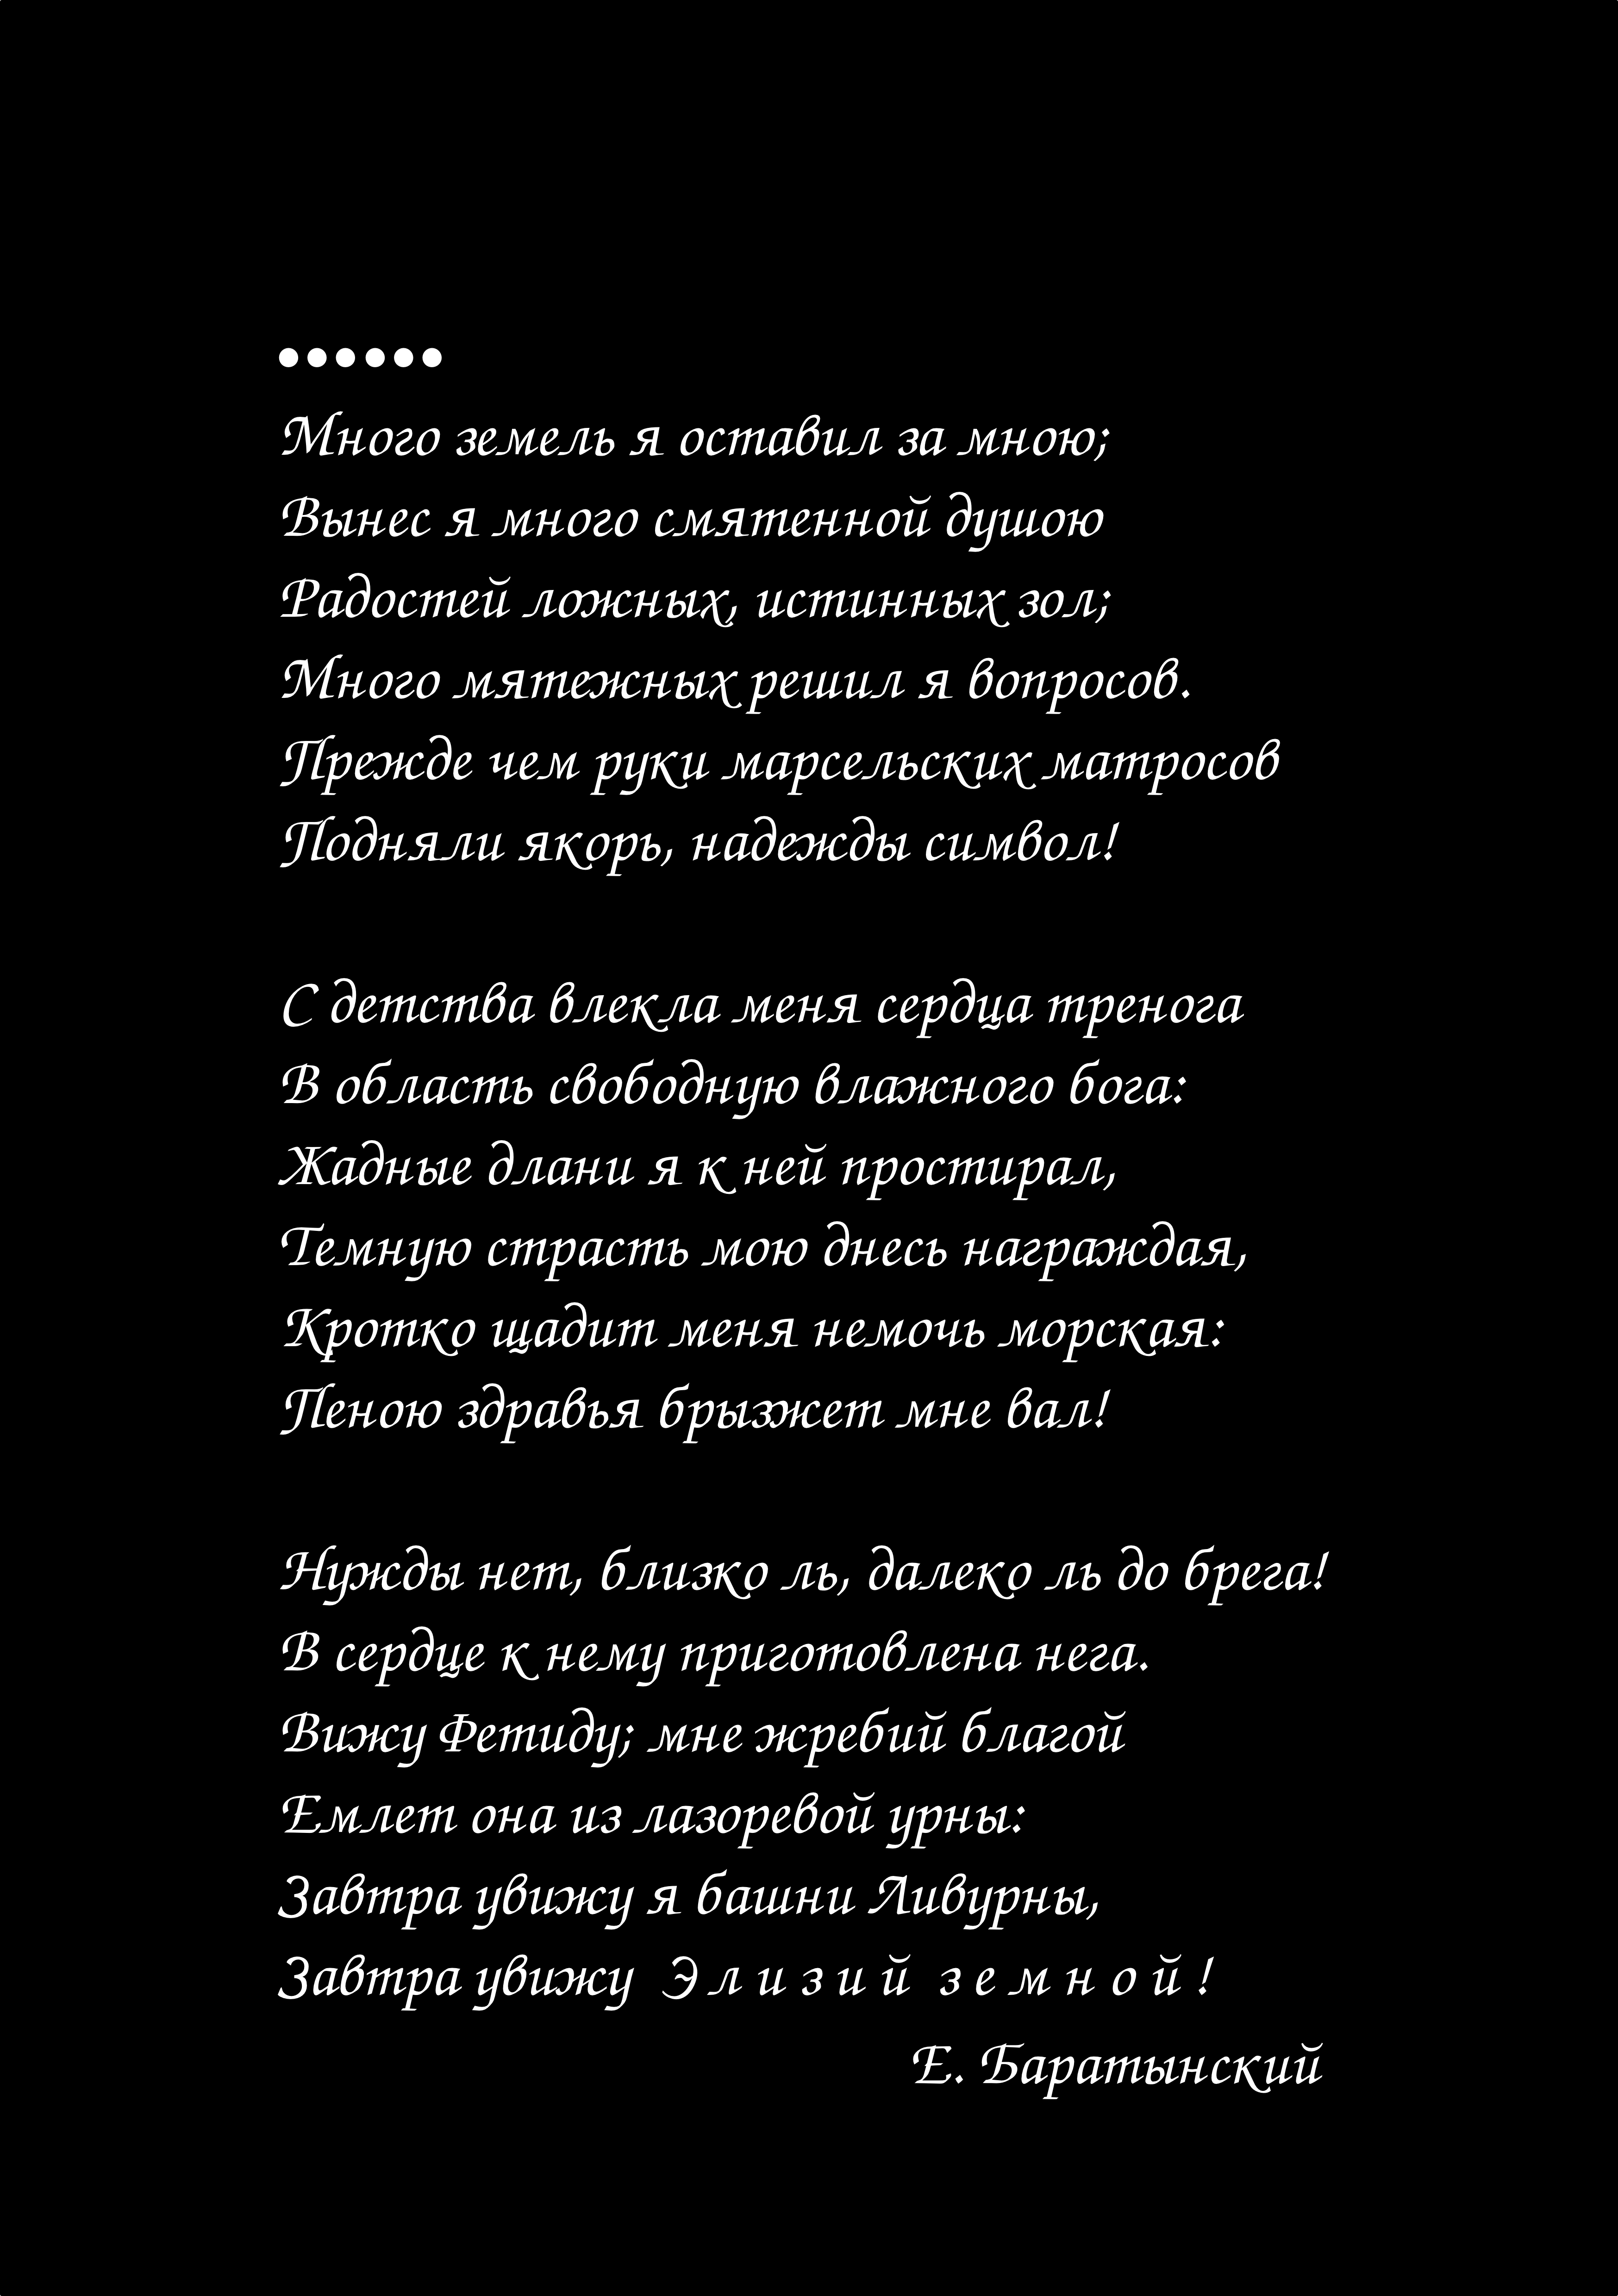
\includegraphics[width=1\linewidth]{picts/pyroskaf-2.png} 
%%%
%%\end{center}
%%\end{figure}
%%\newpage

%%\begin{figure}[H]
%%\begin{center}
%%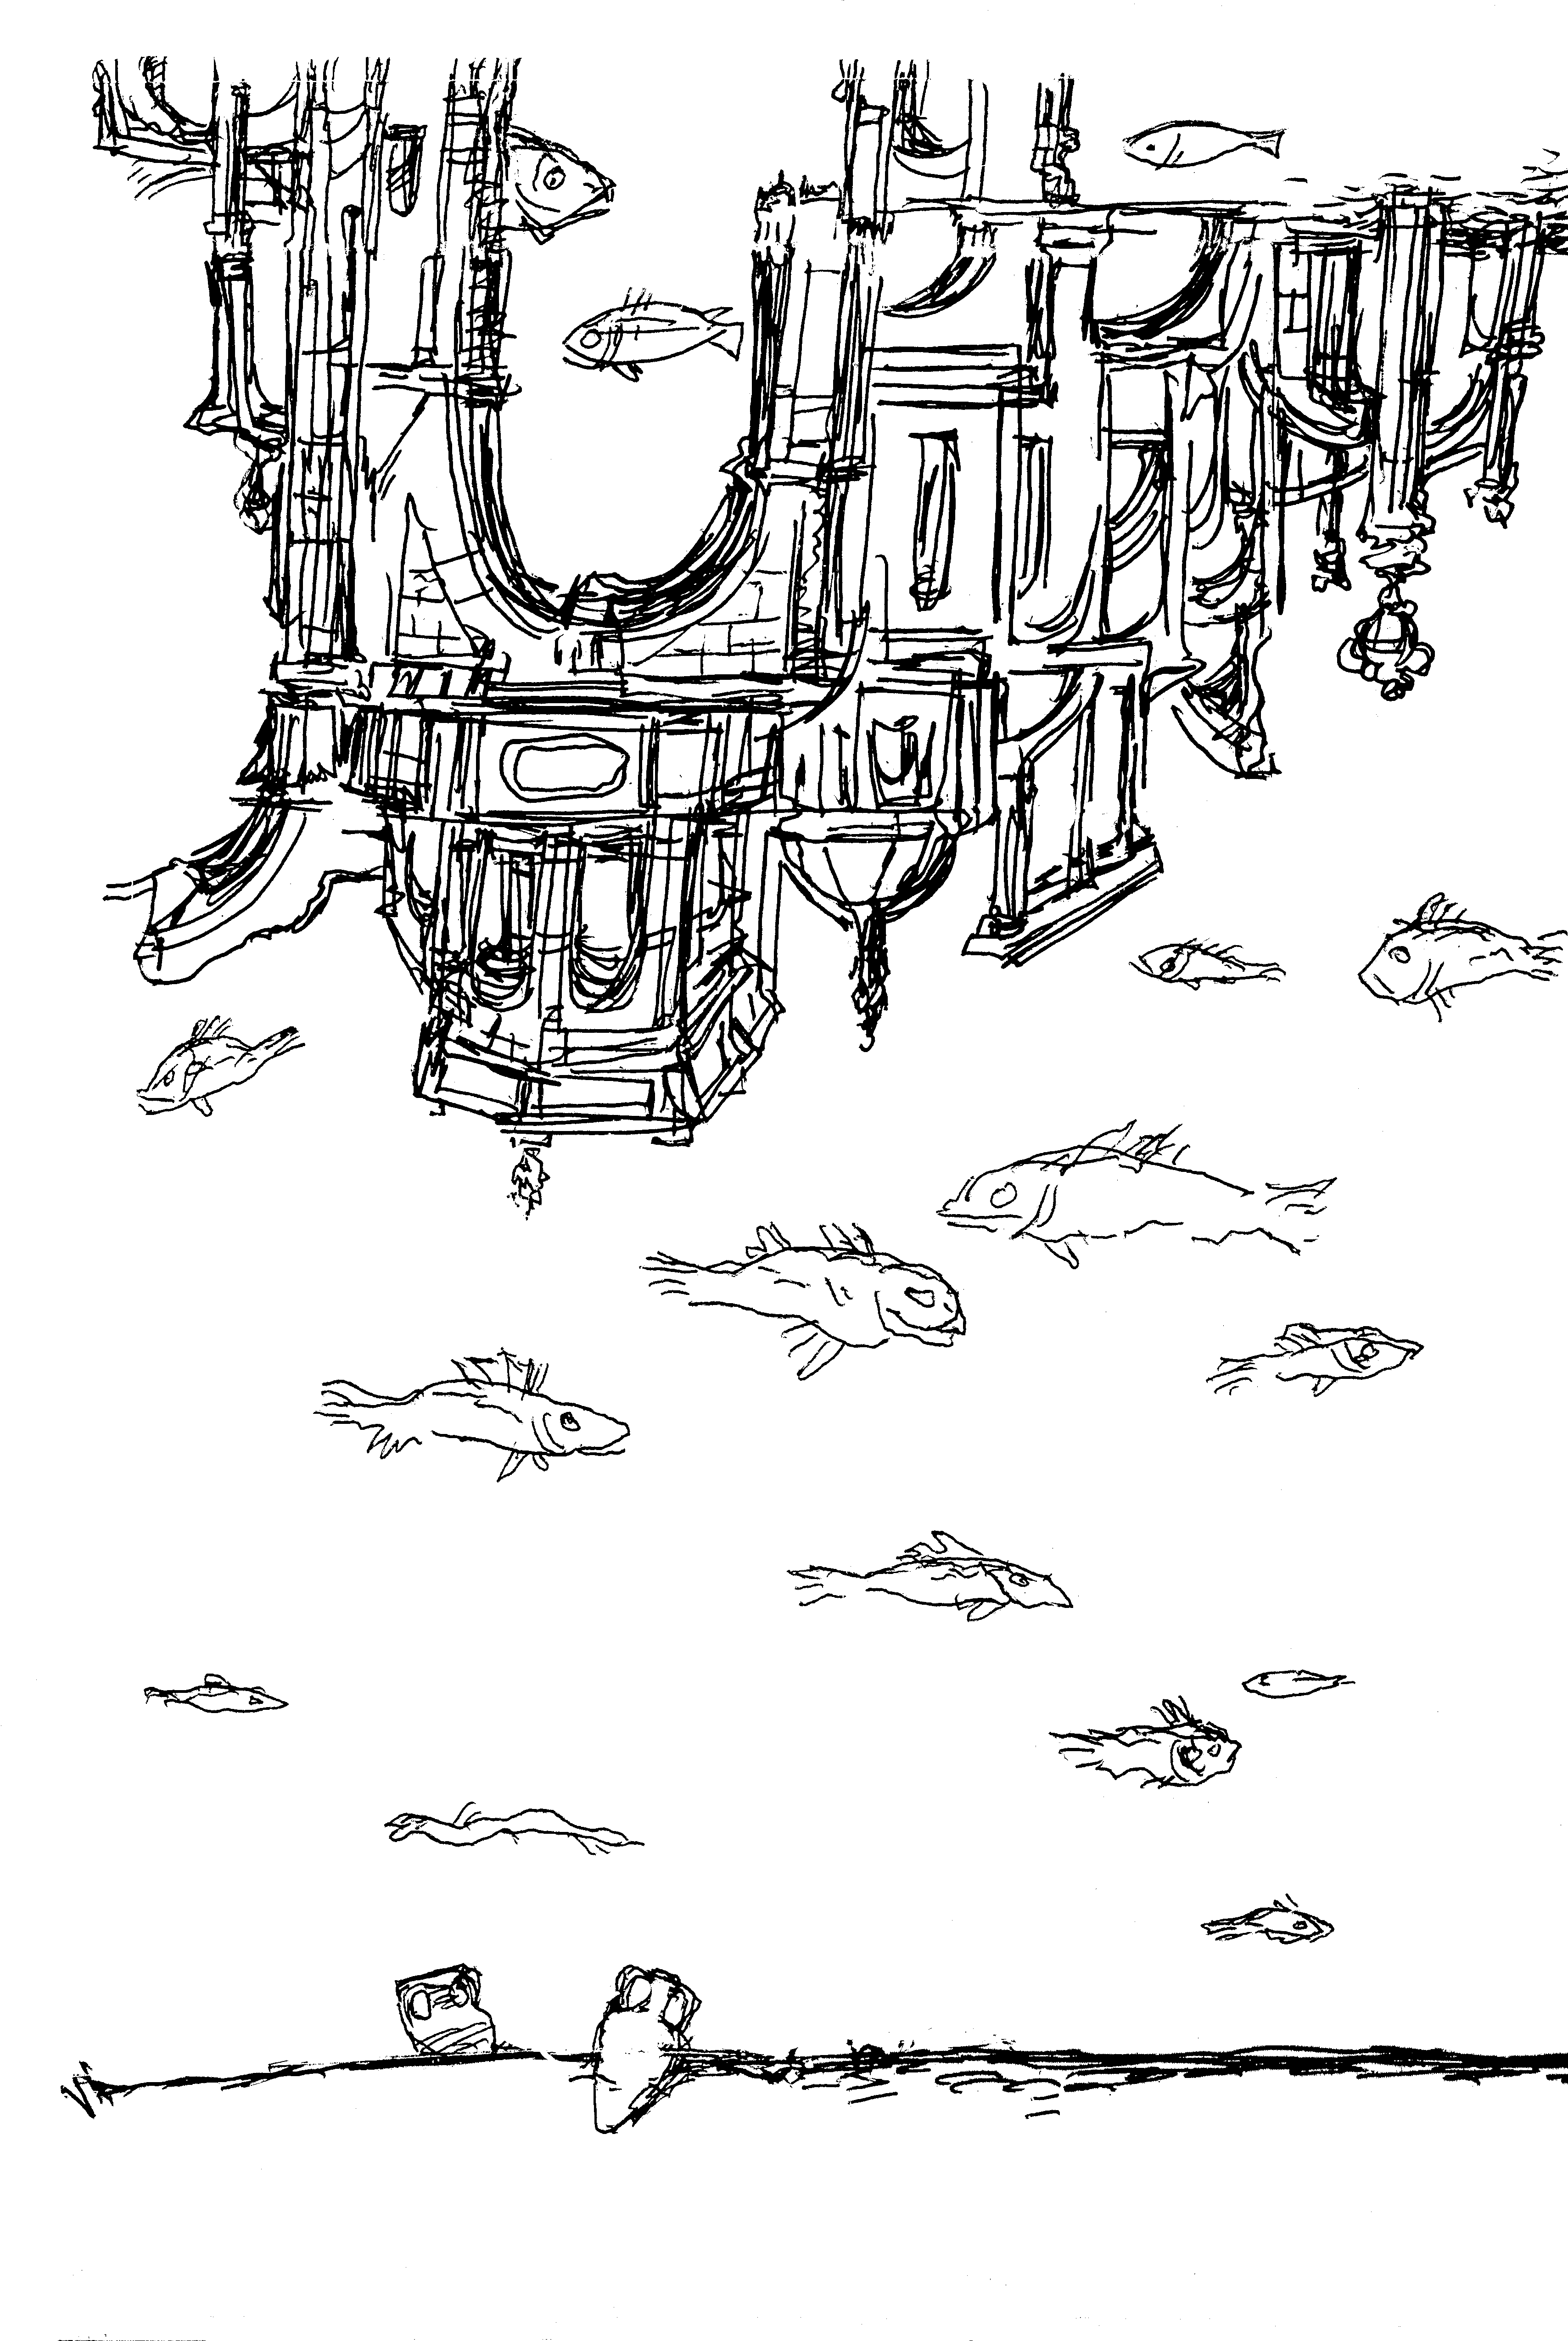
\includegraphics[width=1\linewidth]{picts/oblogka2.png} 
%%%
%%\end{center}
%%\end{figure}
%%\newpage
\twocolumn
\pagestyle{empty}
\small
\tableofcontents

\end{document}
